\chapter{Design}

This section outlines the initial designs for the system to be produced. As this project is being developed using a Scrum based development methodology, there is no concrete up front design for the system. Much of the design presented here was created during the initial stages of the project and therefore has been subject to change throughout the implementation stages of the project. However, we were not going to start development on the project without any design whatsoever, especially since nearly all team members were unfamiliar with the technologies we were going to be working with. Unless otherwise stated all designs are applicable to both the .NET and Java EE systems.

\section{Use Case Diagrams}

The first real piece of design to be undertaken was a detailed analysis of the requirements specification. This initial step aimed to tease out what was likely to be the most challenging, unintuitive elements of the project. Through this discussion we were able to draw out what we thought were the major use cases for the different system users.

Figure \ref{fig:use-case-login} shows the use cases for registering and logging in a user to the system. Note that all types of the system user can perform these actions regardless of their role. By ``vanilla'' login/registration we mean a custom login system specific to the site that does not interact with another site via SSO etc.

Figure \ref{fig:use-case-account-admin} shows the different actions that can be performed to administer a user account with the GoAber system. These are mostly common sense and would be the sort of actions normally expected of system such as this. Note that in figure \ref{fig:use-case-account-admin} administrators can do everything a participant can plus modifying their privileges. Changing user privileges is the only action that cannot be performed by anyone other than an administrator. ``Deactivating'' a user account will leave an audit record in the system but will remove all activity data as well. 

\begin{figure}[H]
\centering
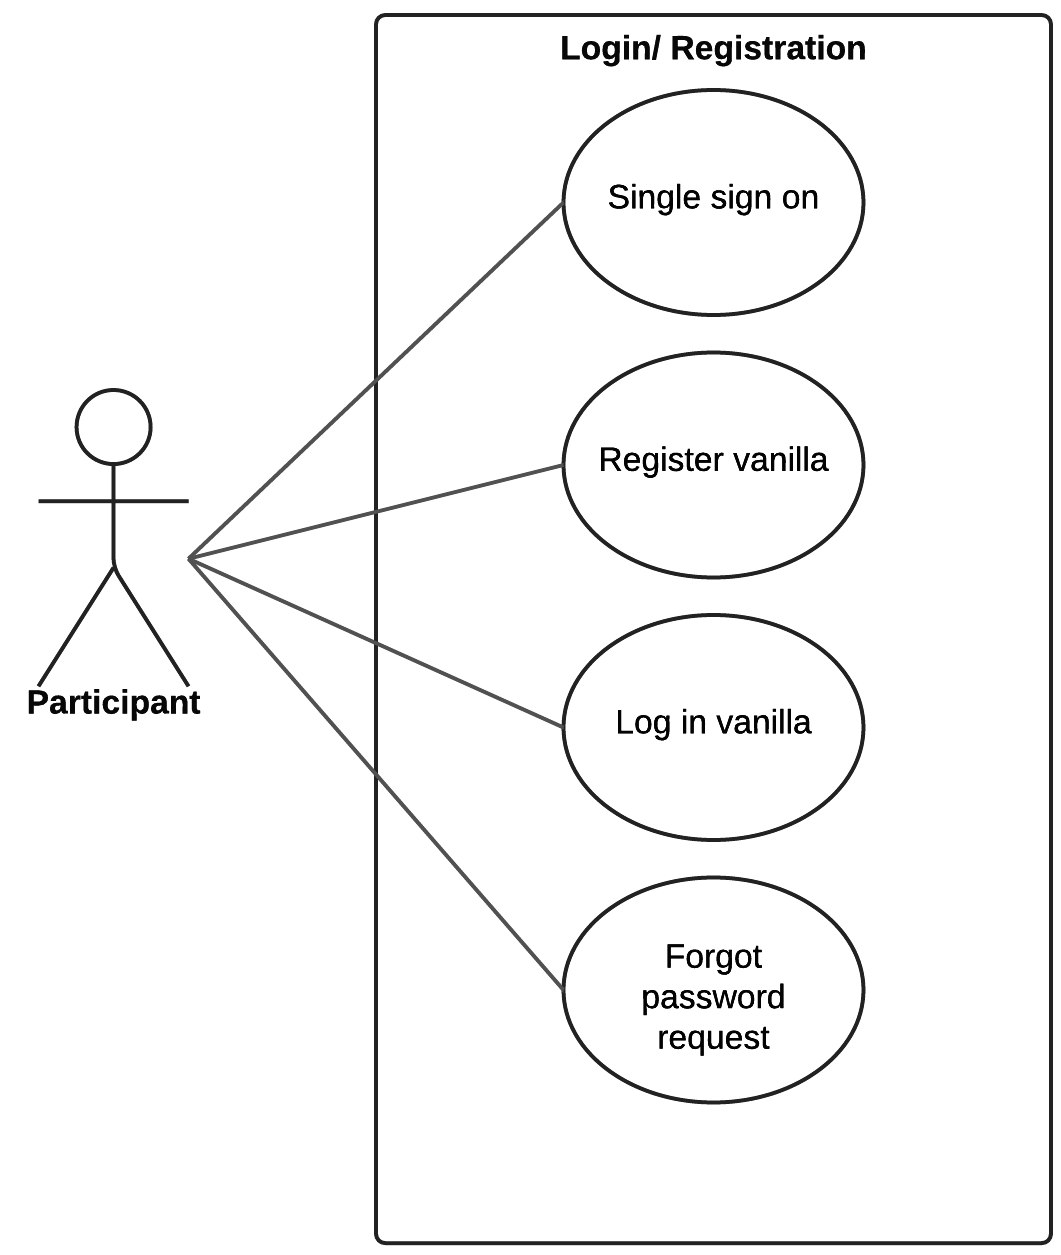
\includegraphics[width=0.5\textwidth]{../design/UML/UseCase/Login-Register.png}
\caption{Shows the different login \& registration actions that a system user (participant, coordinator or administrator) can take. These actions are associated with D-FR11.}
\label{fig:use-case-login}
\end{figure}

\begin{figure}[H]
\centering
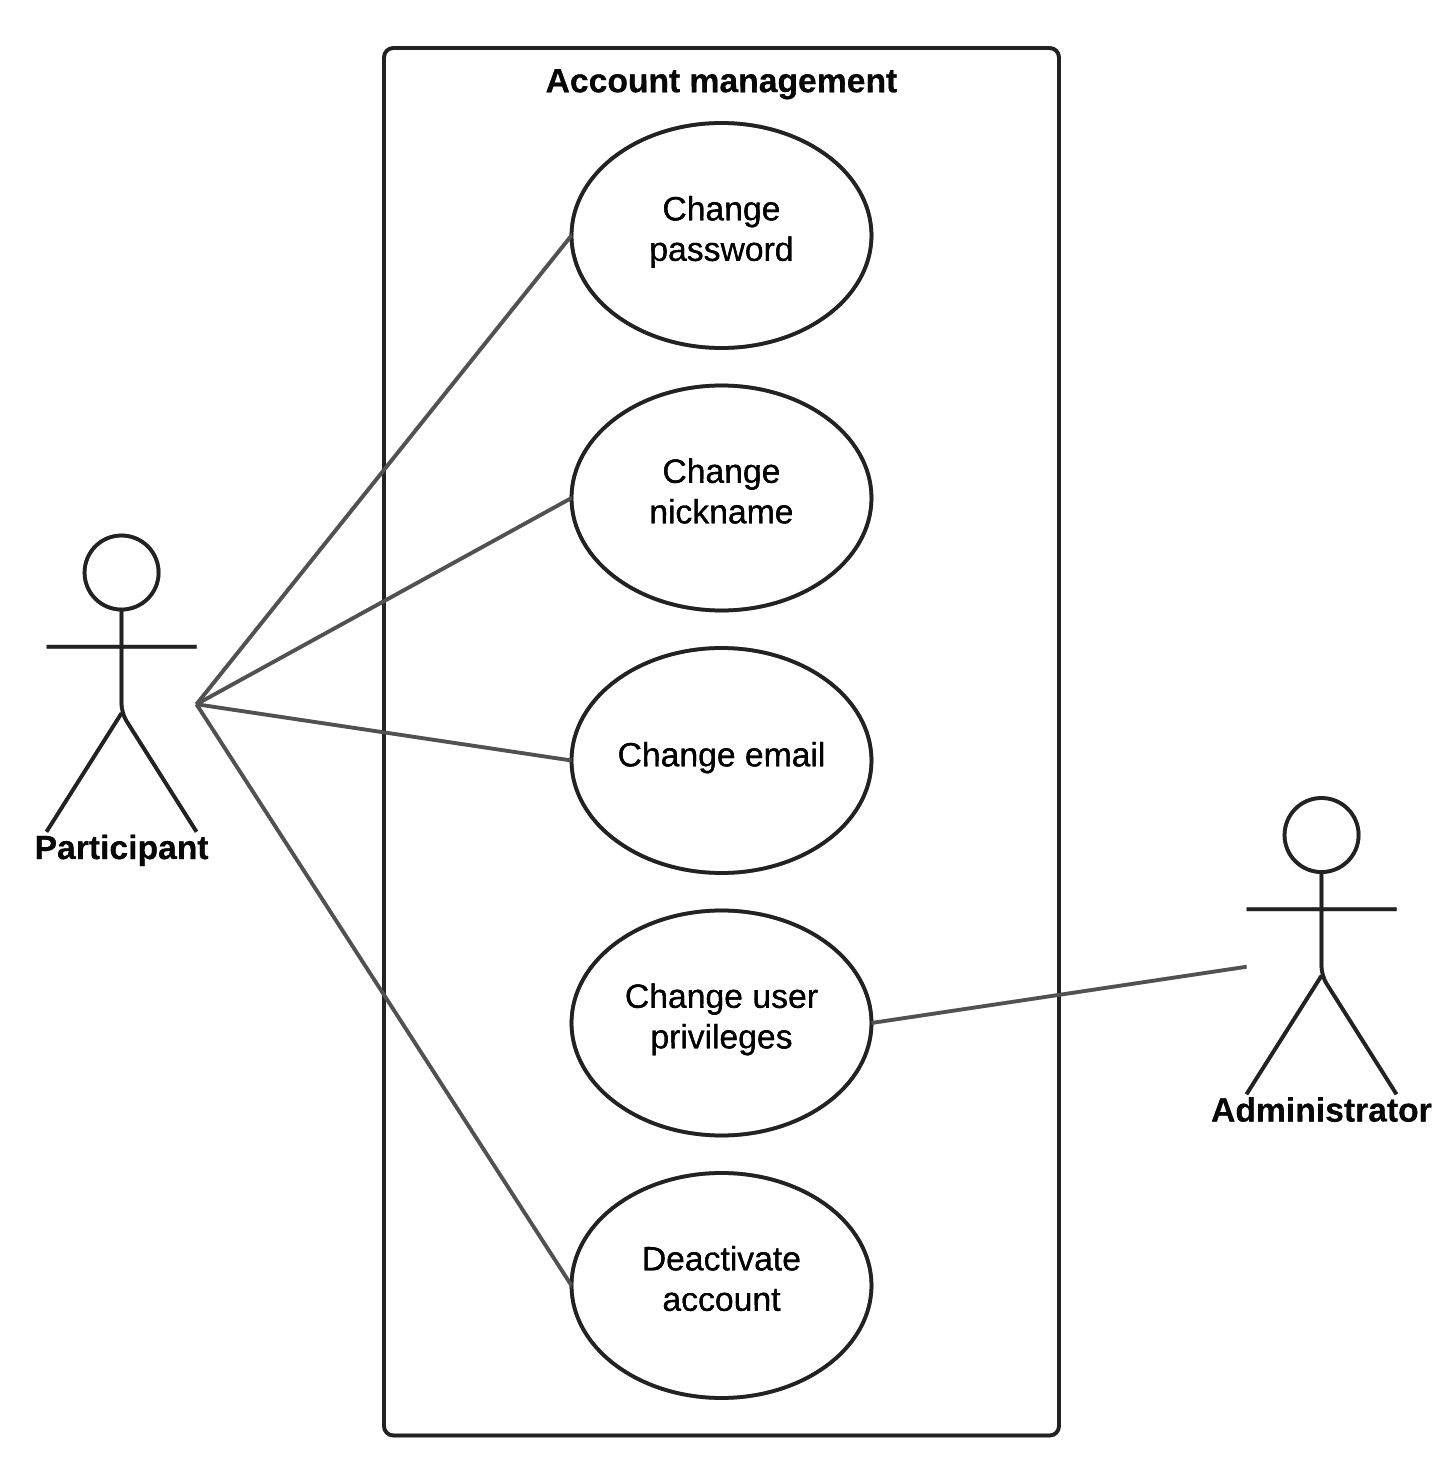
\includegraphics[width=0.6\textwidth]{../design/UML/UseCase/Account-Management.png}
\caption{Shows the different account administration actions that can be performed by a participant of the system. This references requirements D-FR1 and D-FR10.}
\label{fig:use-case-account-admin}
\end{figure}

The next use case diagram (figure \ref{fig:use-case-activity-data}) is arguably the most important in the series. This gives a loose summary of how the users will interact with their activity data in the system. It also shows which actors have permission to carry out particular actions. As mentioned before, administrators can carry out all actions that co-ordinators and participants can. Co-ordinators can only view information about themselves and others, much in the same way as users, but can obviously perform CRUD actions on their own data.

The diagram shown in figure \ref{fig:use-case-group} shows the interactions that can be carried out on groups of users. Administrators have the permission to perform CRUD operations on a group and have the ability to add participants to a group. Participants are only able to view a summary of other people in the group.

\begin{figure}[H]
\centering
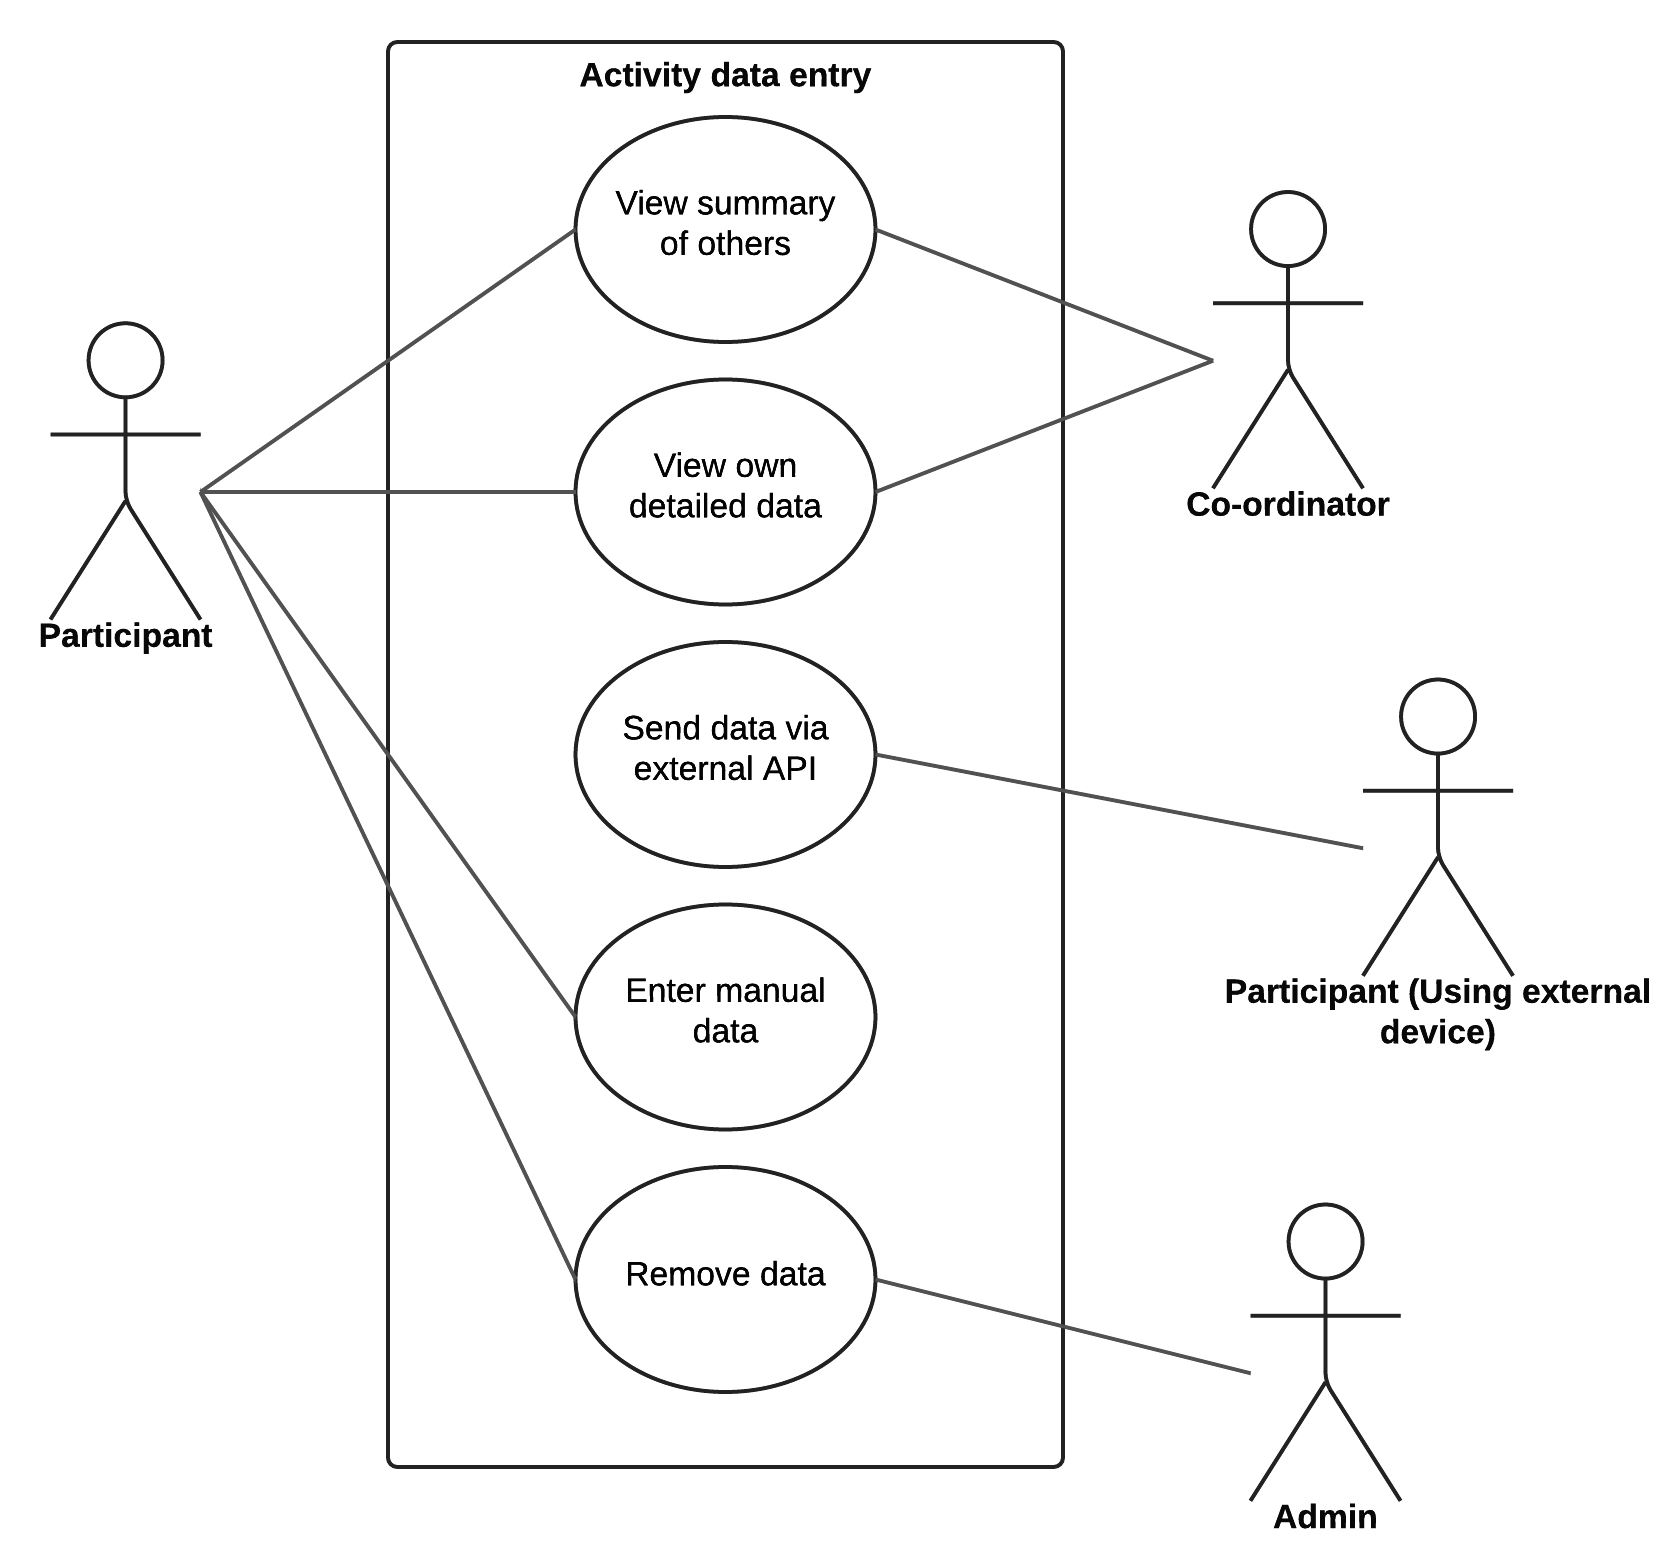
\includegraphics[width=0.6\textwidth]{../design/UML/UseCase/Participant-Activity-Data.png}
\caption{Shows the actions that can be performed by the three types on activity data. These were taken from requirements D-FR5, 7, 8, 9, 10}
\label{fig:use-case-activity-data}
\end{figure}

\begin{figure}[H]
\centering
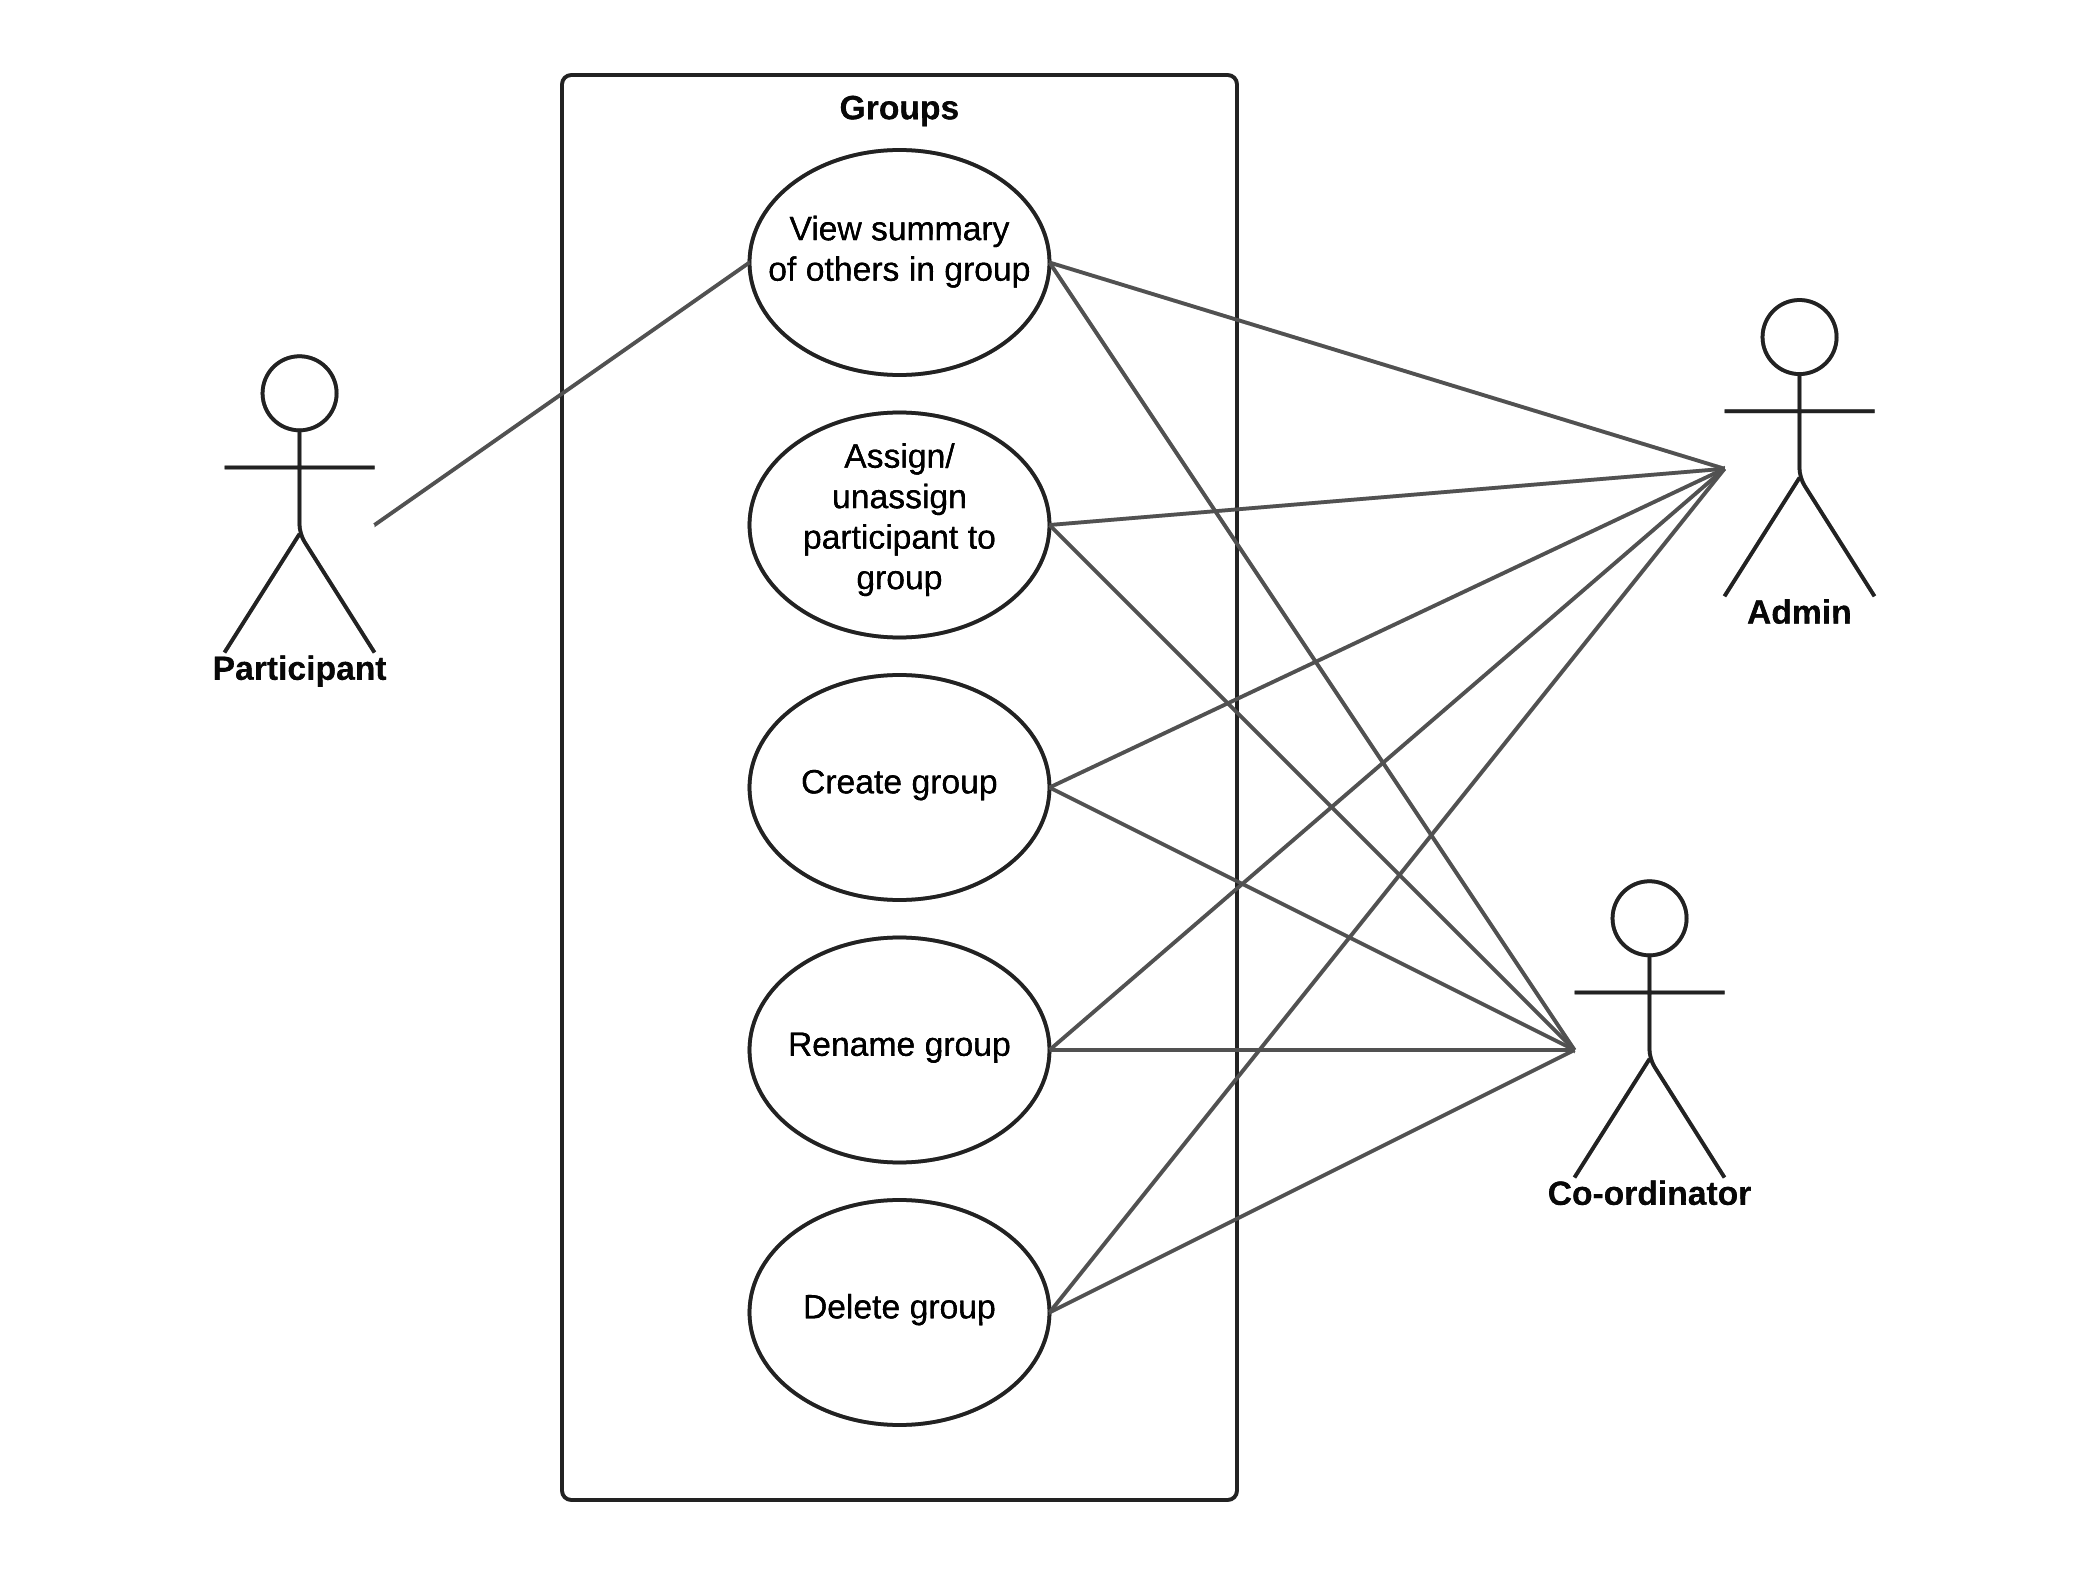
\includegraphics[width=0.7\textwidth]{../design/UML/UseCase/Groups.png}
\caption{Shows how actors will interact with groups of users. This is in relation to requirements D-FR1, D-FR10}
\label{fig:use-case-group}
\end{figure}

Use cases for challenges are shown in figure \ref{fig:use-case-challenges}. Here, the major differences to be aware of are the differences between what actions a user and coordinator can perform. Users can only view information about challenges while coordinators can setup and edit challenges between groups and communities. Administrators will be able to perform all of these actions.

Figure \ref{fig:use-case-assigning-devices} shows a couple of additional participant use cases which will be required in order to allow users to authorise their devices with our system. Participants should be able to authorise their devices another system via OAuth.


\begin{figure}[H]
\centering
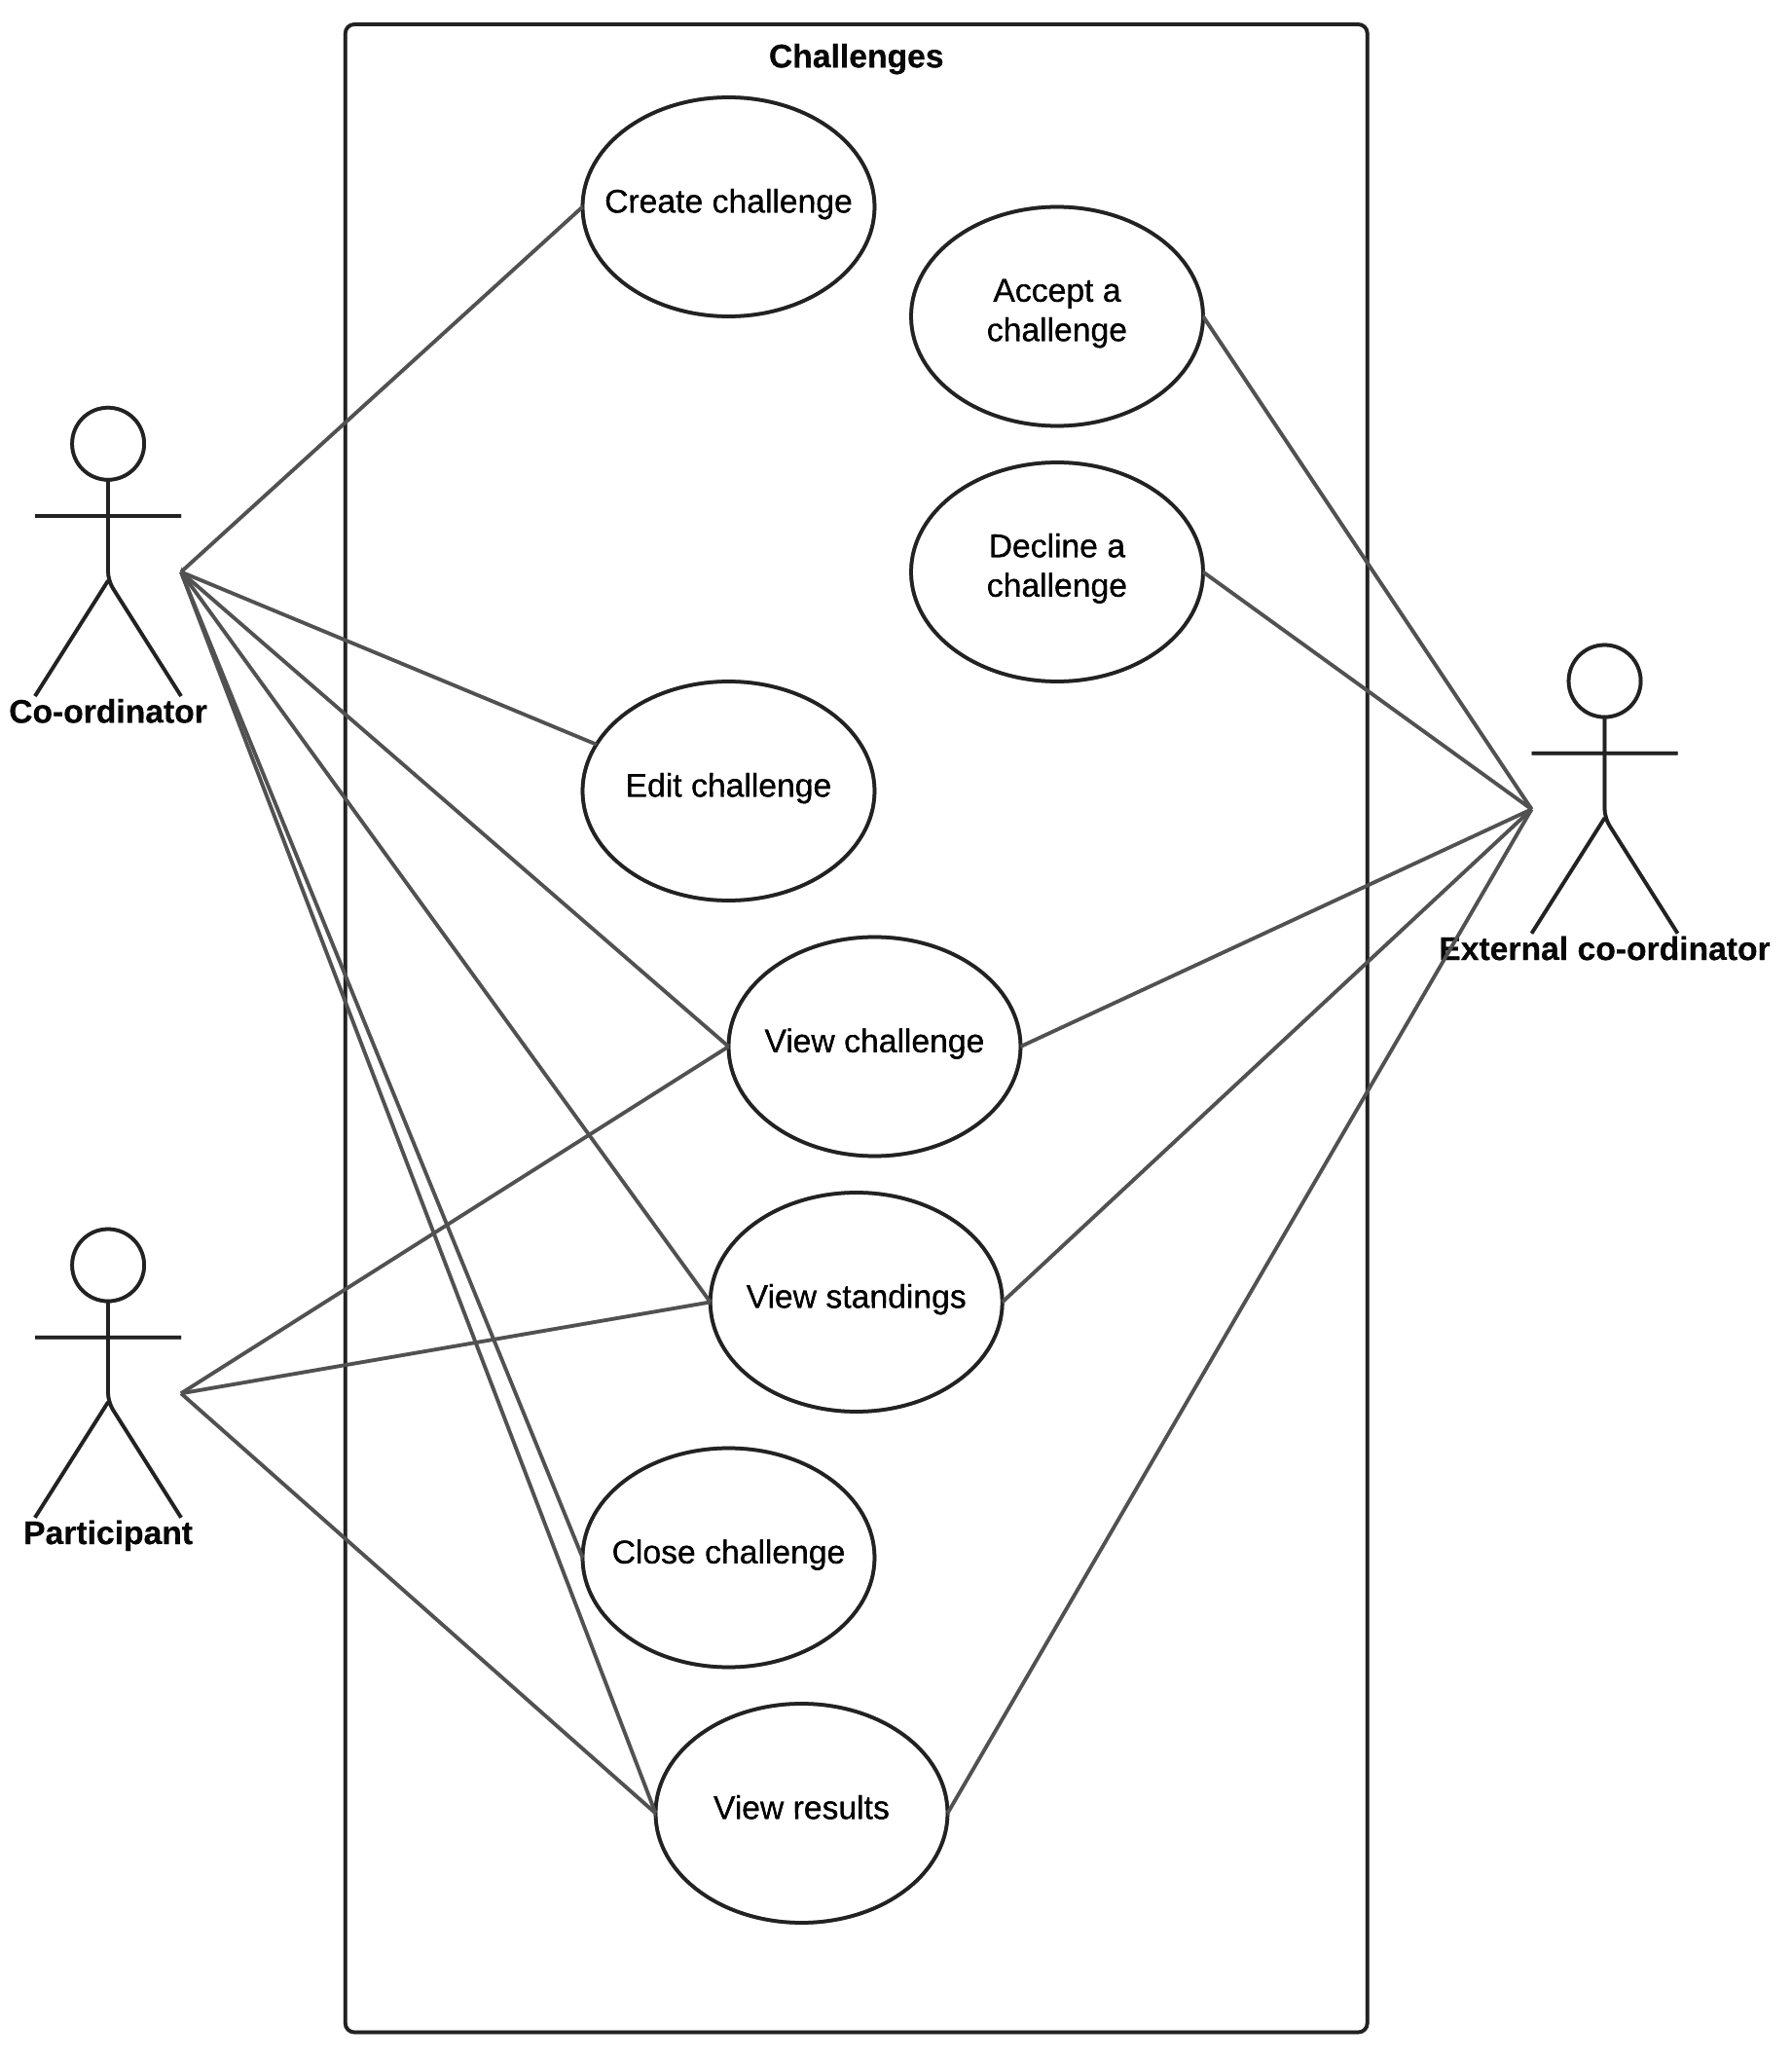
\includegraphics[width=0.6\textwidth]{../design/UML/UseCase/Challenges.png}
\caption{Shows how actors will interact with the system in terms of challenges. These reference requirements C-FR1-4 and E-FR1}
\label{fig:use-case-challenges}
\end{figure}

\begin{figure}[H]
\centering
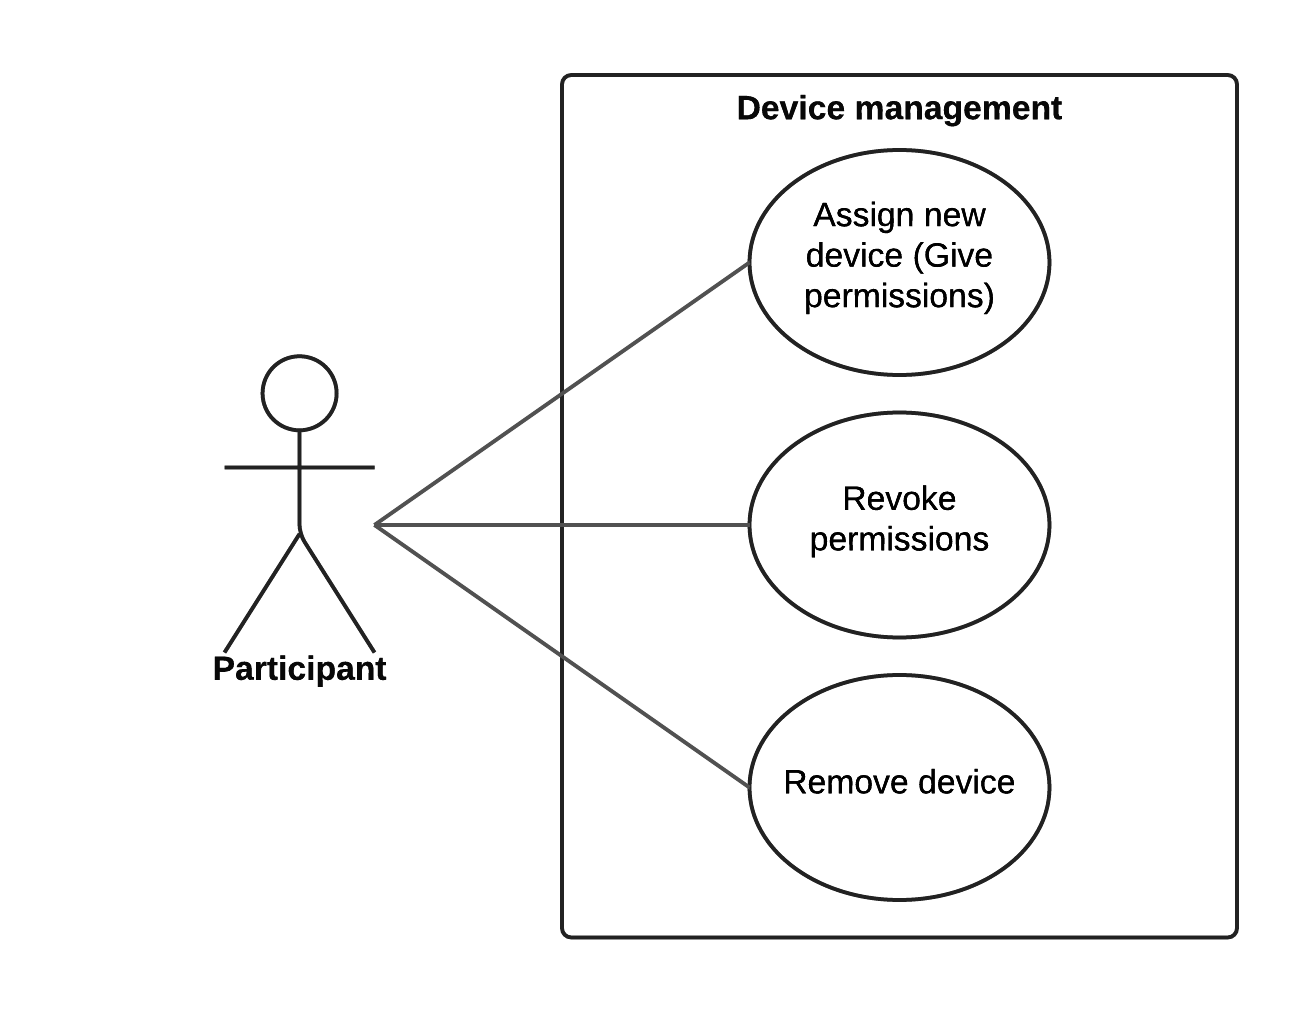
\includegraphics[width=0.6\textwidth]{../design/UML/UseCase/Assigning-Devices.png}
\caption{Shows how a user can authorise a device with an external system (e.g. Jawbone/Fitbit). This relates to requirement D-FR3.}
\label{fig:use-case-assigning-devices}
\end{figure}

Finally, figure \ref{fig:use-case-admin-settings} shows some additional use cases for system administrators. This figure simply states some additional actions which were not included in the other use case diagrams. Administrators should be able to schedule the emails that get sent out from the system as well as edit and delete users.

\begin{figure}[H]
\centering
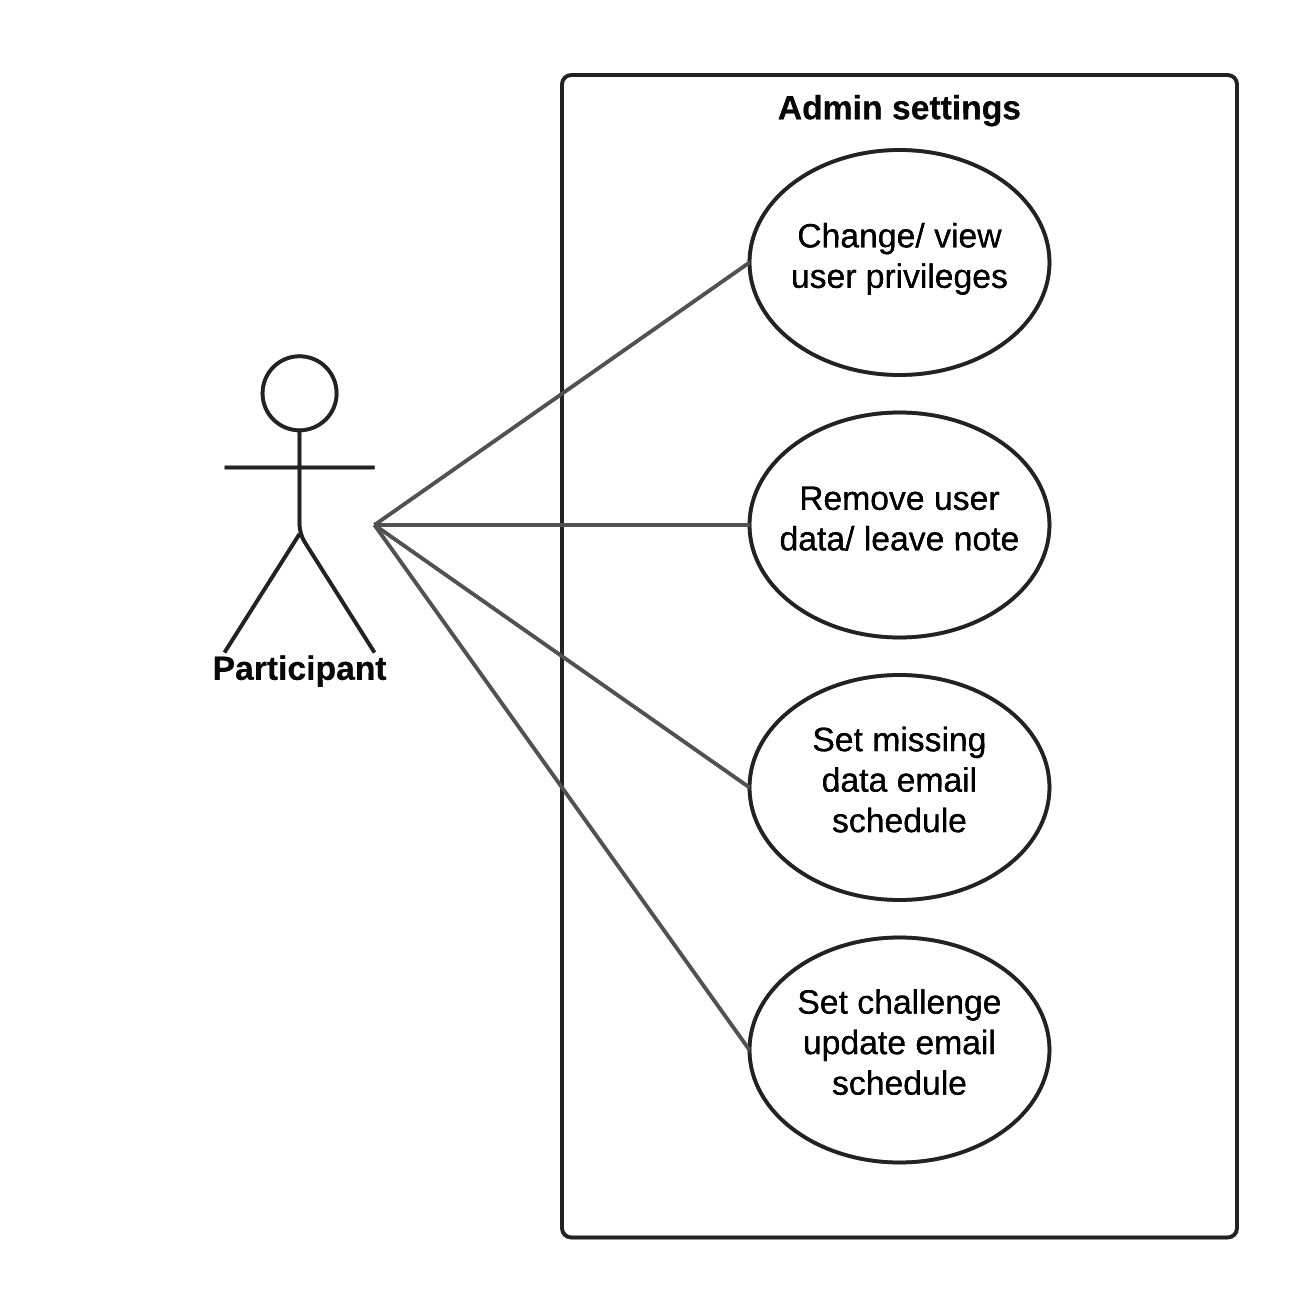
\includegraphics[width=0.6\textwidth]{../design/UML/UseCase/Admin-Settings.png}
\caption{Shows some additional uses cases that can be performed by a system administrator. These action are all taken from requirements D-FR1, D-FR8, E-FR3 and E-FR4.}
\label{fig:use-case-admin-settings}
\end{figure}

\section{System Architecture}
This section discussed the high level system architecture that we conceived in the very early stages of the project. Figure \ref{fig:system-architecture} shows a formalised version of the early system architecture. We in no way expect the final design of the implemented system to accurately reflect this diagram. This diagram was a useful by product of early discussions to try and understand how the final system might hang to together. This was a key discussion that lead to us identifying parts of the system that we did not readily understand or that we found to be ambiguous. 

This design was originally produced in rough on a white board, allowing us to  shuffle key elements around until we were in agreement on how each part should work. Afterwards the diagram was formalised into figure \ref{fig:system-architecture} to be preserved as a design artefact. This overview is meant to be independent of the technology used (either .NET or JavaEE). This, combined with the fact that a Scrum based methodology can and will allow us to be flexible with the design are the major reasons why the final system will almost inevitably differ from this diagram. However, as mentioned, it played an important role in getting all team members on the same page before diving into implementation.

The system in diagram \ref{fig:system-architecture} can be split into two parts: ``our system'' on the left hand side and the ``outside world'' on the right. The outside world consists of regular human users (participants, coordinators, and administrators) but also includes other computer systems. For example, other GoAber systems need to communicate information about users and challenges between one another. Other systems that need to be communicated with are the Fitbit/Jawbone servers and with generic SOAP input.

The diagram shows several connections from our system to the outside world. The most obvious one, in the top centre of the diagram, shows that users can connect to a front end website. Conceptually this component is broken down into two parts: the views (what the page looks like) and the controllers (how the views get displayed). The models sit further back in the system and are accessed by the controllers.

Below this component is the SOAP web API. This provides an access point for remote systems (i.e. non-human users) to communicate with our system. This includes both other community servers and potential other devices.

The third point of access in the bottom centre of the diagram is the most complicated part of the external communication systems. This shows a scheduling component, inside of which is nested a data collection component. The scheduling component will be responsible for firing off events both internally and externally. For example, internally this will be responsible for closing a challenge on time. Externally it will be used to periodically request data from the Fitbit and Jawbone APIs and as a timer to send out emails.

Sitting behind these front three layers are the business logic and data models for the system. These are shared by all three of the components described above. This part of the diagram is deliberately left more vague than the other parts of the diagram. As mentioned in the preceding chapter, we are using a Scrum based methodology and producing a big up front design would be going against its guidelines. Additionally this section of the system is highly likely to be specific to .NET and Java EE. For this reason we will choose to keep the low level design decisions of this part of the system up to the developer. Broadly speaking our approach in this project will be to keep the .NET and Java EE systems structured similarly. Both systems should share the same model structures, unless the specific implementation forces us to change for some reason.

\begin{figure}[H]
\centering
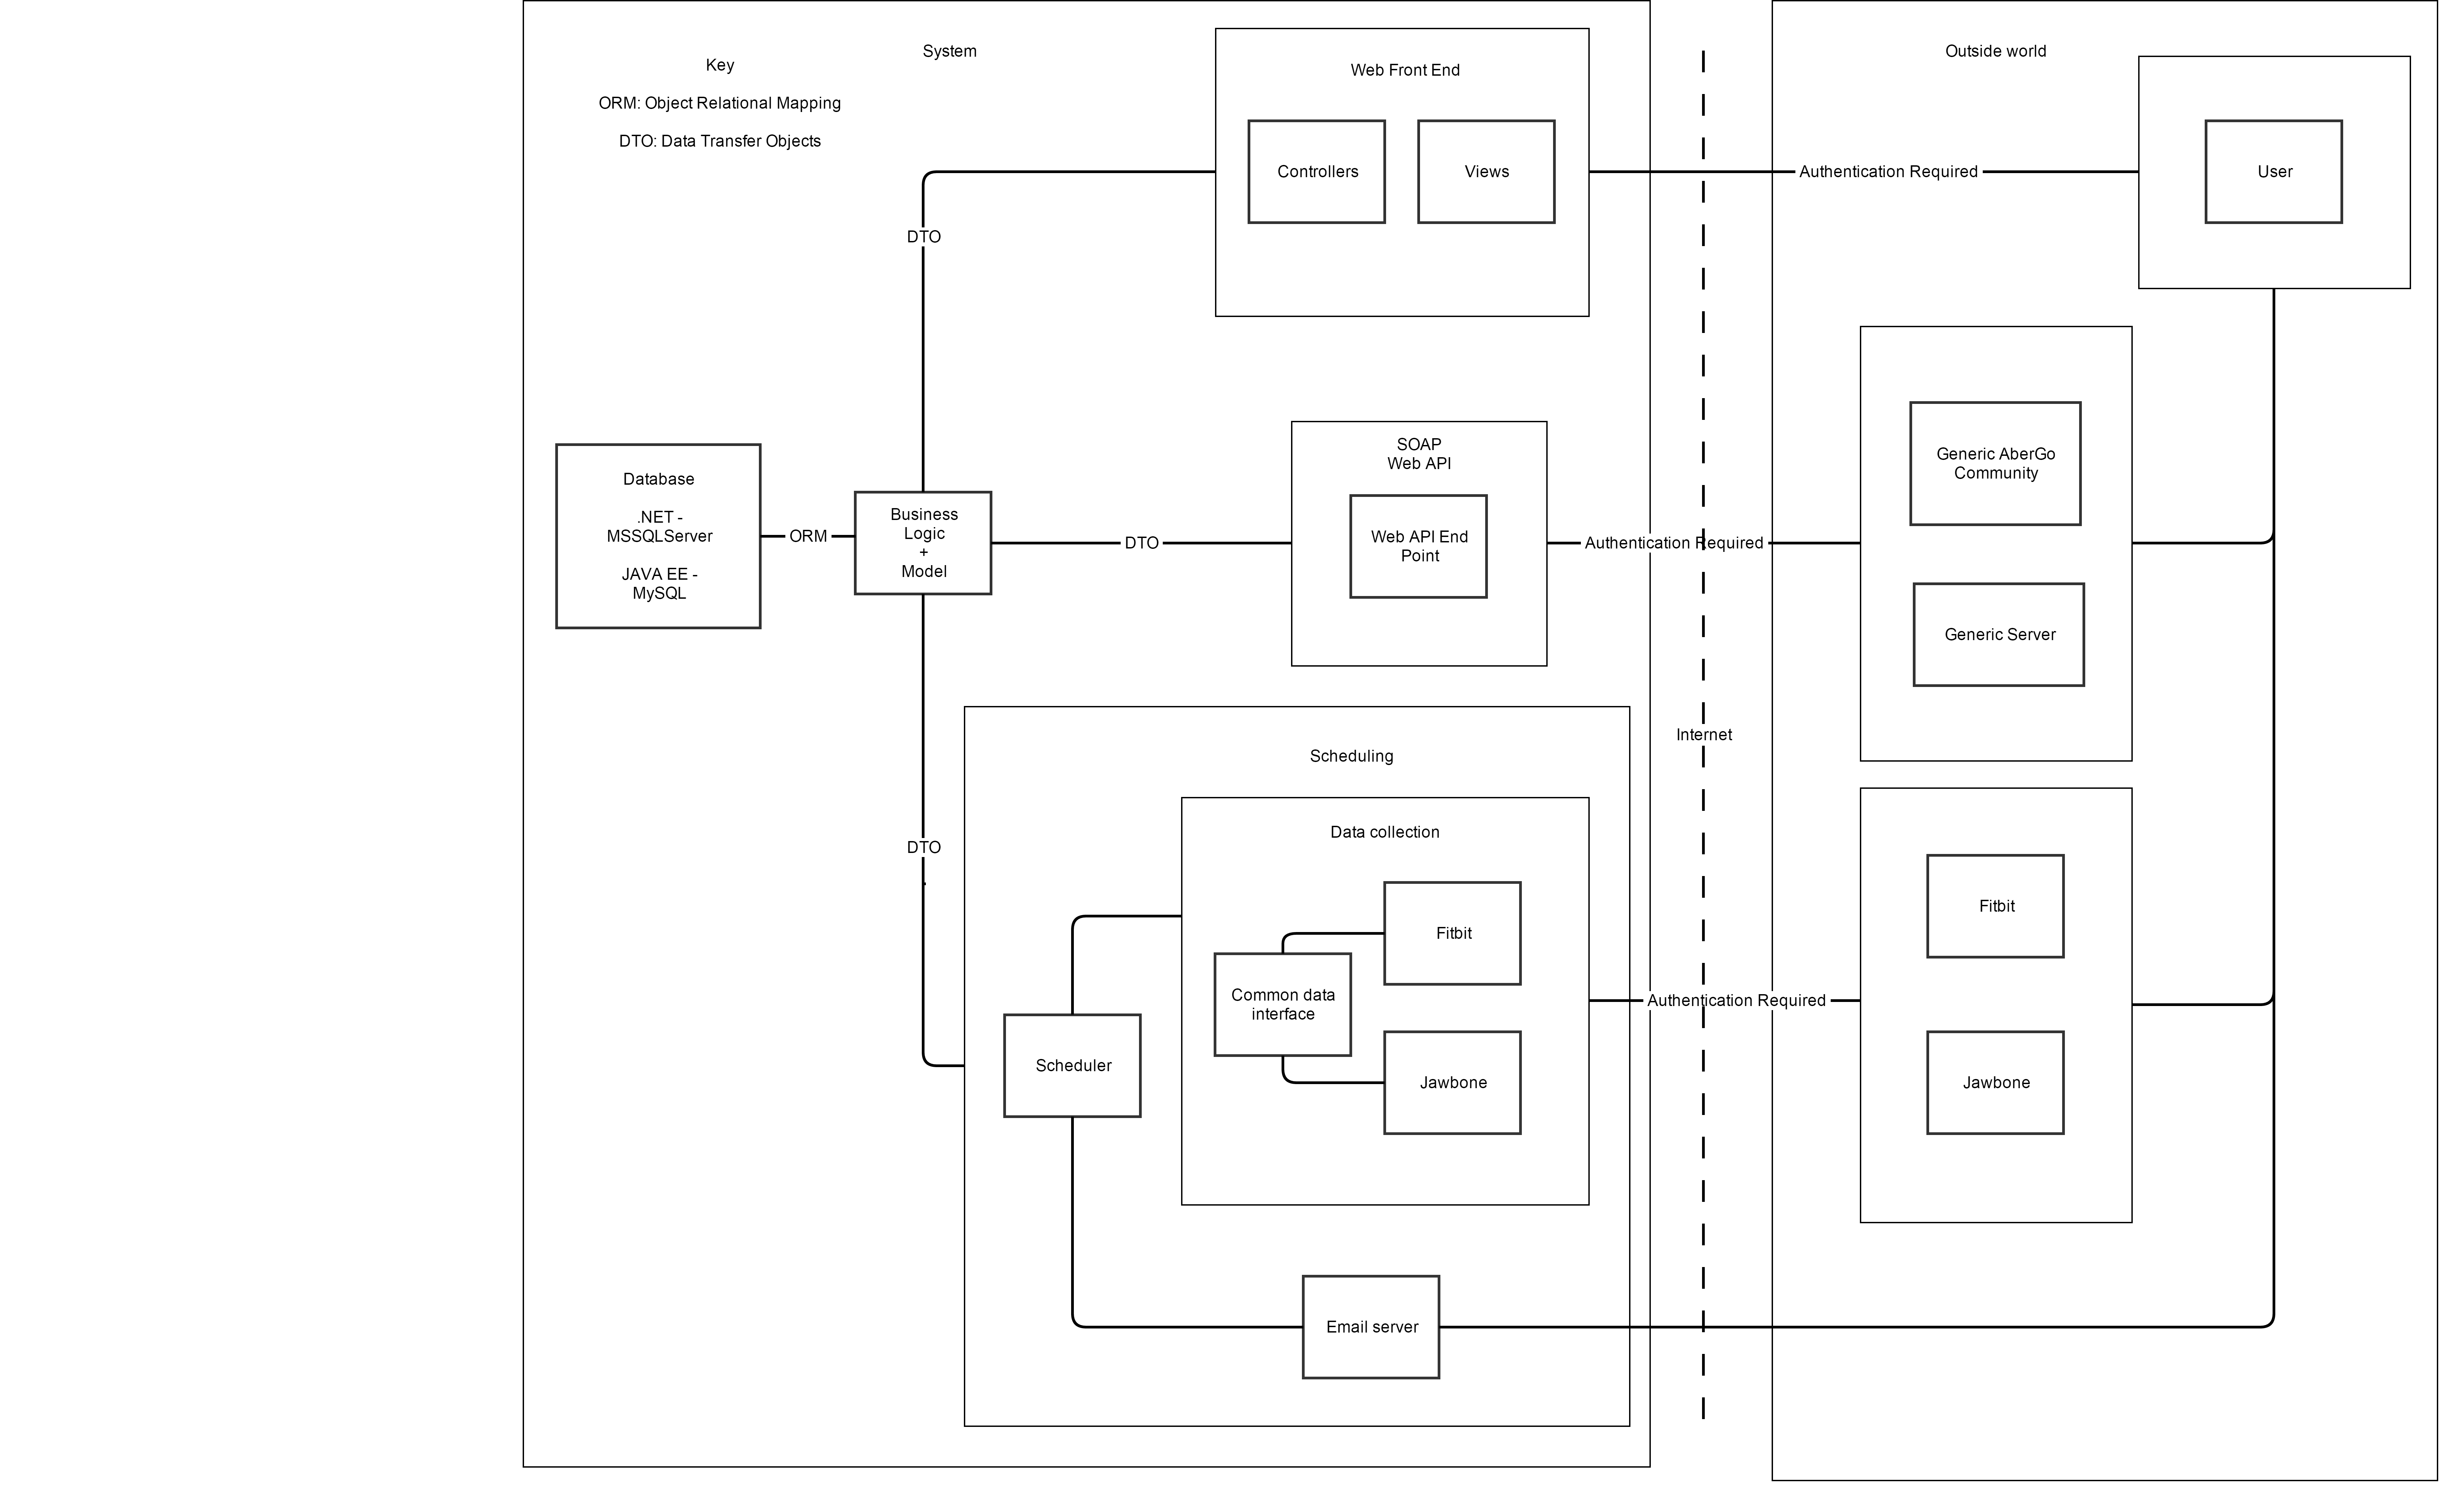
\includegraphics[width=1.0\textwidth]{../design/system/groupproject_systemarchitecture.png}
\caption{High level conceptual overview of the proposed system.}
\label{fig:system-architecture}
\end{figure}

\section{Database Design}
The second major piece of design that we undertook in preparation for the implementation of this project was to come up with an entity relationship diagram which would form the basis for the model code in both versions of the application. Once again, in practice it is likely that this design will need to change once we become more familiar with the two different technologies we are using.

This, like the high system architecture in the previous section was very important to do early on in the project. It helped to solidify how we were going to represent data in our system and gave good starting guidelines for the team members who implement these designs.

Starting to the right of the diagram is the \textit{ActivityData} entity. This is perhaps the most important entity in the entire system. An \textit{ActivityData} item is a single piece of activity data for a particular user. An \textit{ActivityData} entity is associated with a particular system \textit{User} and also has a reference to a \textit{CategoryUnit} entity. A \textit{CategoryUnit} is simply a linking table between the categories (such as ``running'' and ``swimming'') and units (such as ``steps'' or ``strokes'').

The system is designed in this way so that there is decoupling between the value of the data stored in the system and the category or unit it belongs to. Every activity data item will simply be stored as a numerical value. The interpretation of that value is determined by what the associated category or unit is. This allows the database model to be flexible to the number of different types of activity data that the client may wish to store in the system. 

This formulation has several distinct advantages. Firstly with this approach there is no need to introduce null entires into the table as you would have to do the type of the data was store alongside the value itself. Secondly, it means that it would be easy to add the ability to introduce new categories and units should the customer require. Thirdly this makes the system almost completely independent of the type of data that a user might want to store. As long as the activity data item is a numerical value, no changes to the database structure are required to introduce the new type. The only exception to this is if the new type of activity data to be introduced happened to be categorical instead of numerical. But even in this circumstance another table could be easily created (e.g. \textit{CategoricalActivityData}) in order to support it.

Moving onto other parts of the model; in the centre of the diagram is the \textit{User} model. This will store almost all of the information about a user (name, email etc.). A user record also has a link to a user credentials table, which contains their password for the system and other authentication data. Additionally users also have a user role associated with them. The user role specifies what type of user they are and permissions they have (e.g. participant, coordinator or administrator).

Along side this user data a user may also register several devices. The devices entity stores the data about a specific device that a user has connected with the site. Each device has a device type. The device type stores the details for connecting to a specific third party site that can be polled by our code for activity data. In this project those sites will be limited to Fitbit and Jawbone.

The top of the diagram shows the tables that will be required to implement the challenges portion of the system. Each user can be associated with a group. A group of conceptually a list of users. Each group belongs to a single community. Groups can have challenges associated with them. A challenge entity contains information such as the start and end date and the type of activity data that is associated with it. Participants in a challenge are linked using the \textit{UserChallenge} entity.

\begin{figure}[H]
\centering
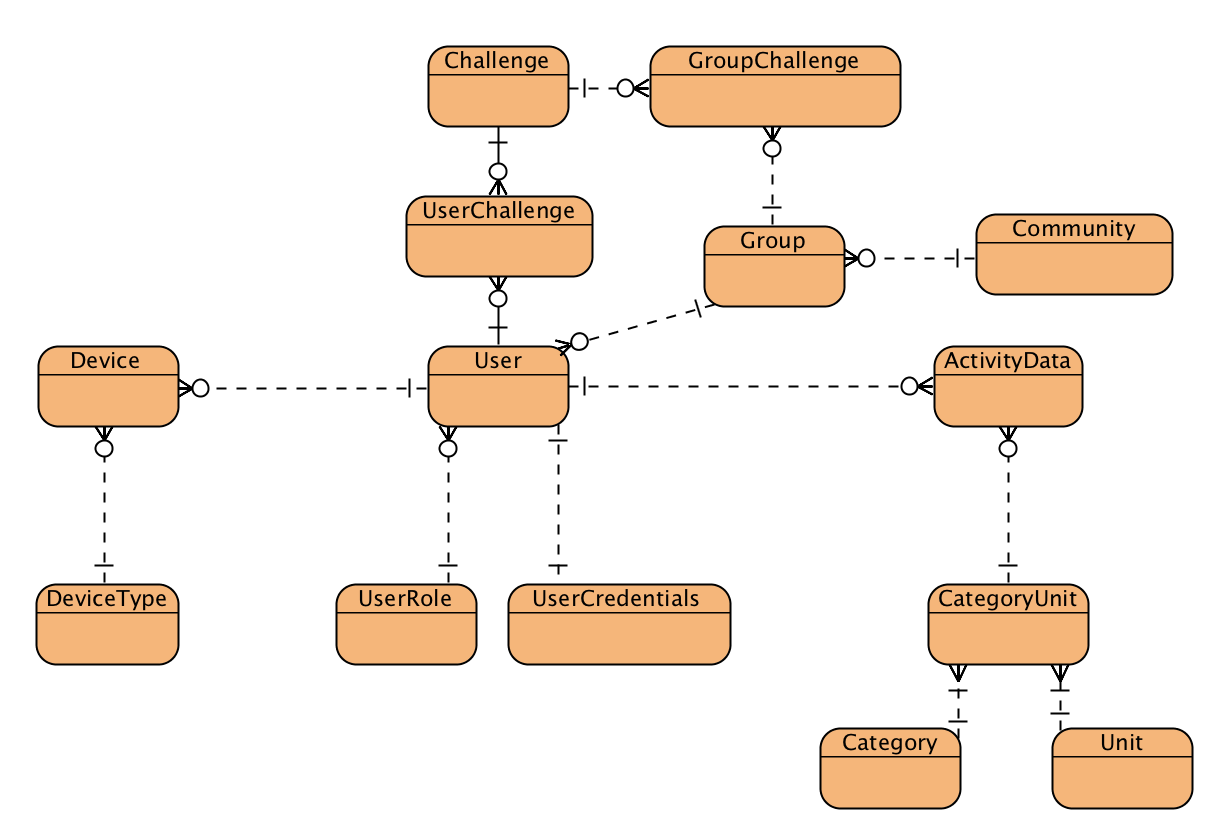
\includegraphics[width=1.0\textwidth]{../design/database/GoAber-ERD.png}
\caption{An entity relationship diagram showing how the data model in both of the applications interact with one another.}
\label{fig:database-design}
\end{figure}

\section{Activity Diagrams}
Alongside the other diagrams presented in this section we also found it useful to produce some state diagrams to try and get a better idea of how a user will transition from one state to another around the site.

Figure \ref{fig:activity-diagram-user-login} shows an activity diagram for authenticating a user in the GoAber system. There are several different paths that a user should be able to follow though the login procedure. If they are already registered they can directly login. If not they must first register with the system before proceeding. In either of these cases if their details fail to validate they are redirected to the appropriate page.

Figure \ref{fig:activity-diagram-accessing-removing-activity-data} shows the workflow for both a participant and an administrator needs to pass through in order to delete activity data from the system. In the case of a participant they should be asked to confirm the deletion. If the user is an administrator they should be also asked to provide a reason for why the data is being removed.

\begin{figure}[H]
\centering
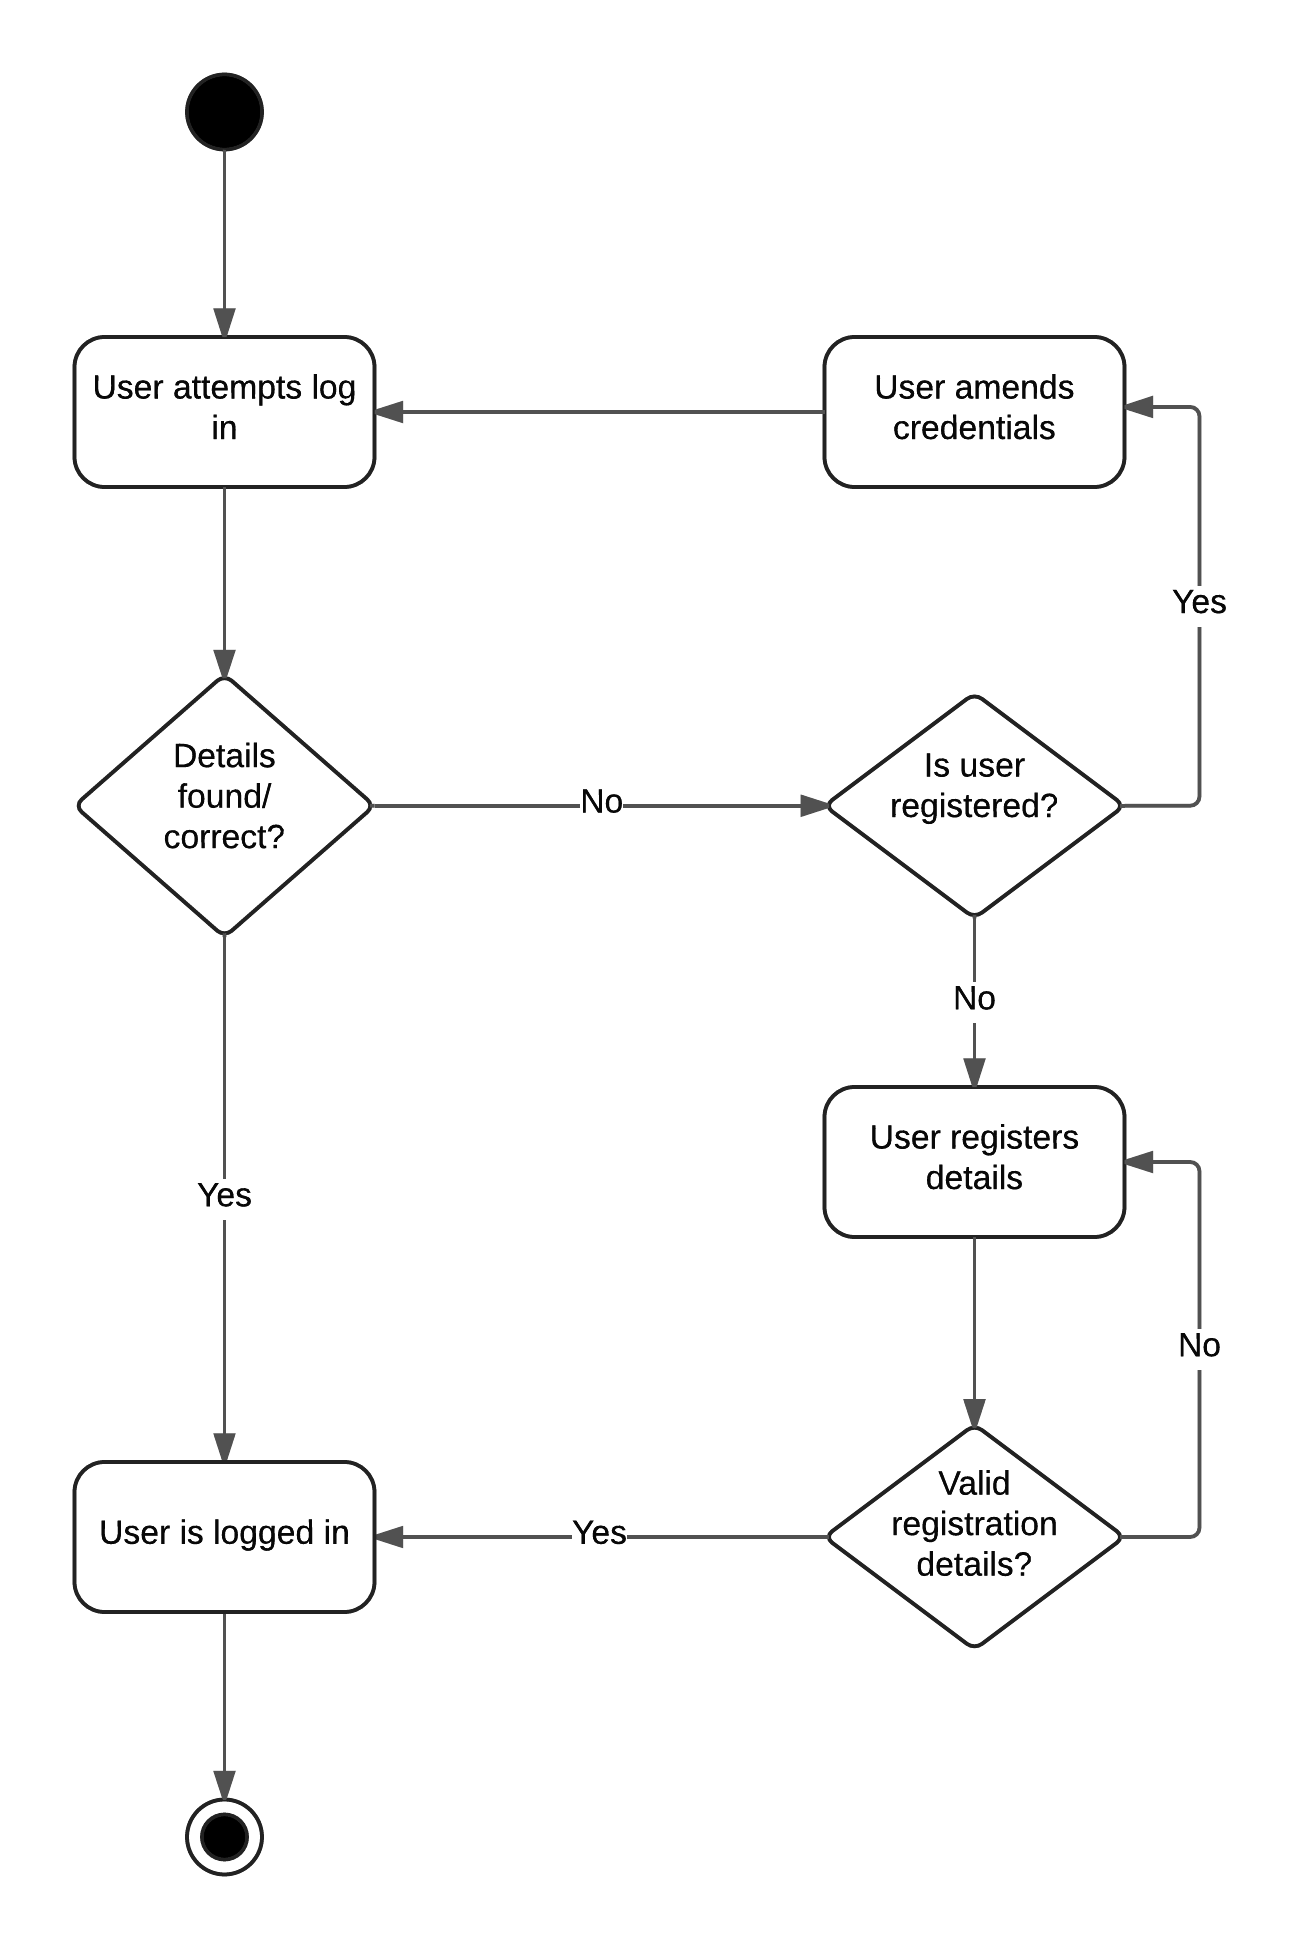
\includegraphics[width=0.4\textwidth]{../design/UML/StateActivity/User-Login-Registration.png}
\caption{An activity diagram showing the states that a user can transition between when authenticating with the system.}
\label{fig:activity-diagram-user-login}
\end{figure}

\begin{figure}[H]
\centering
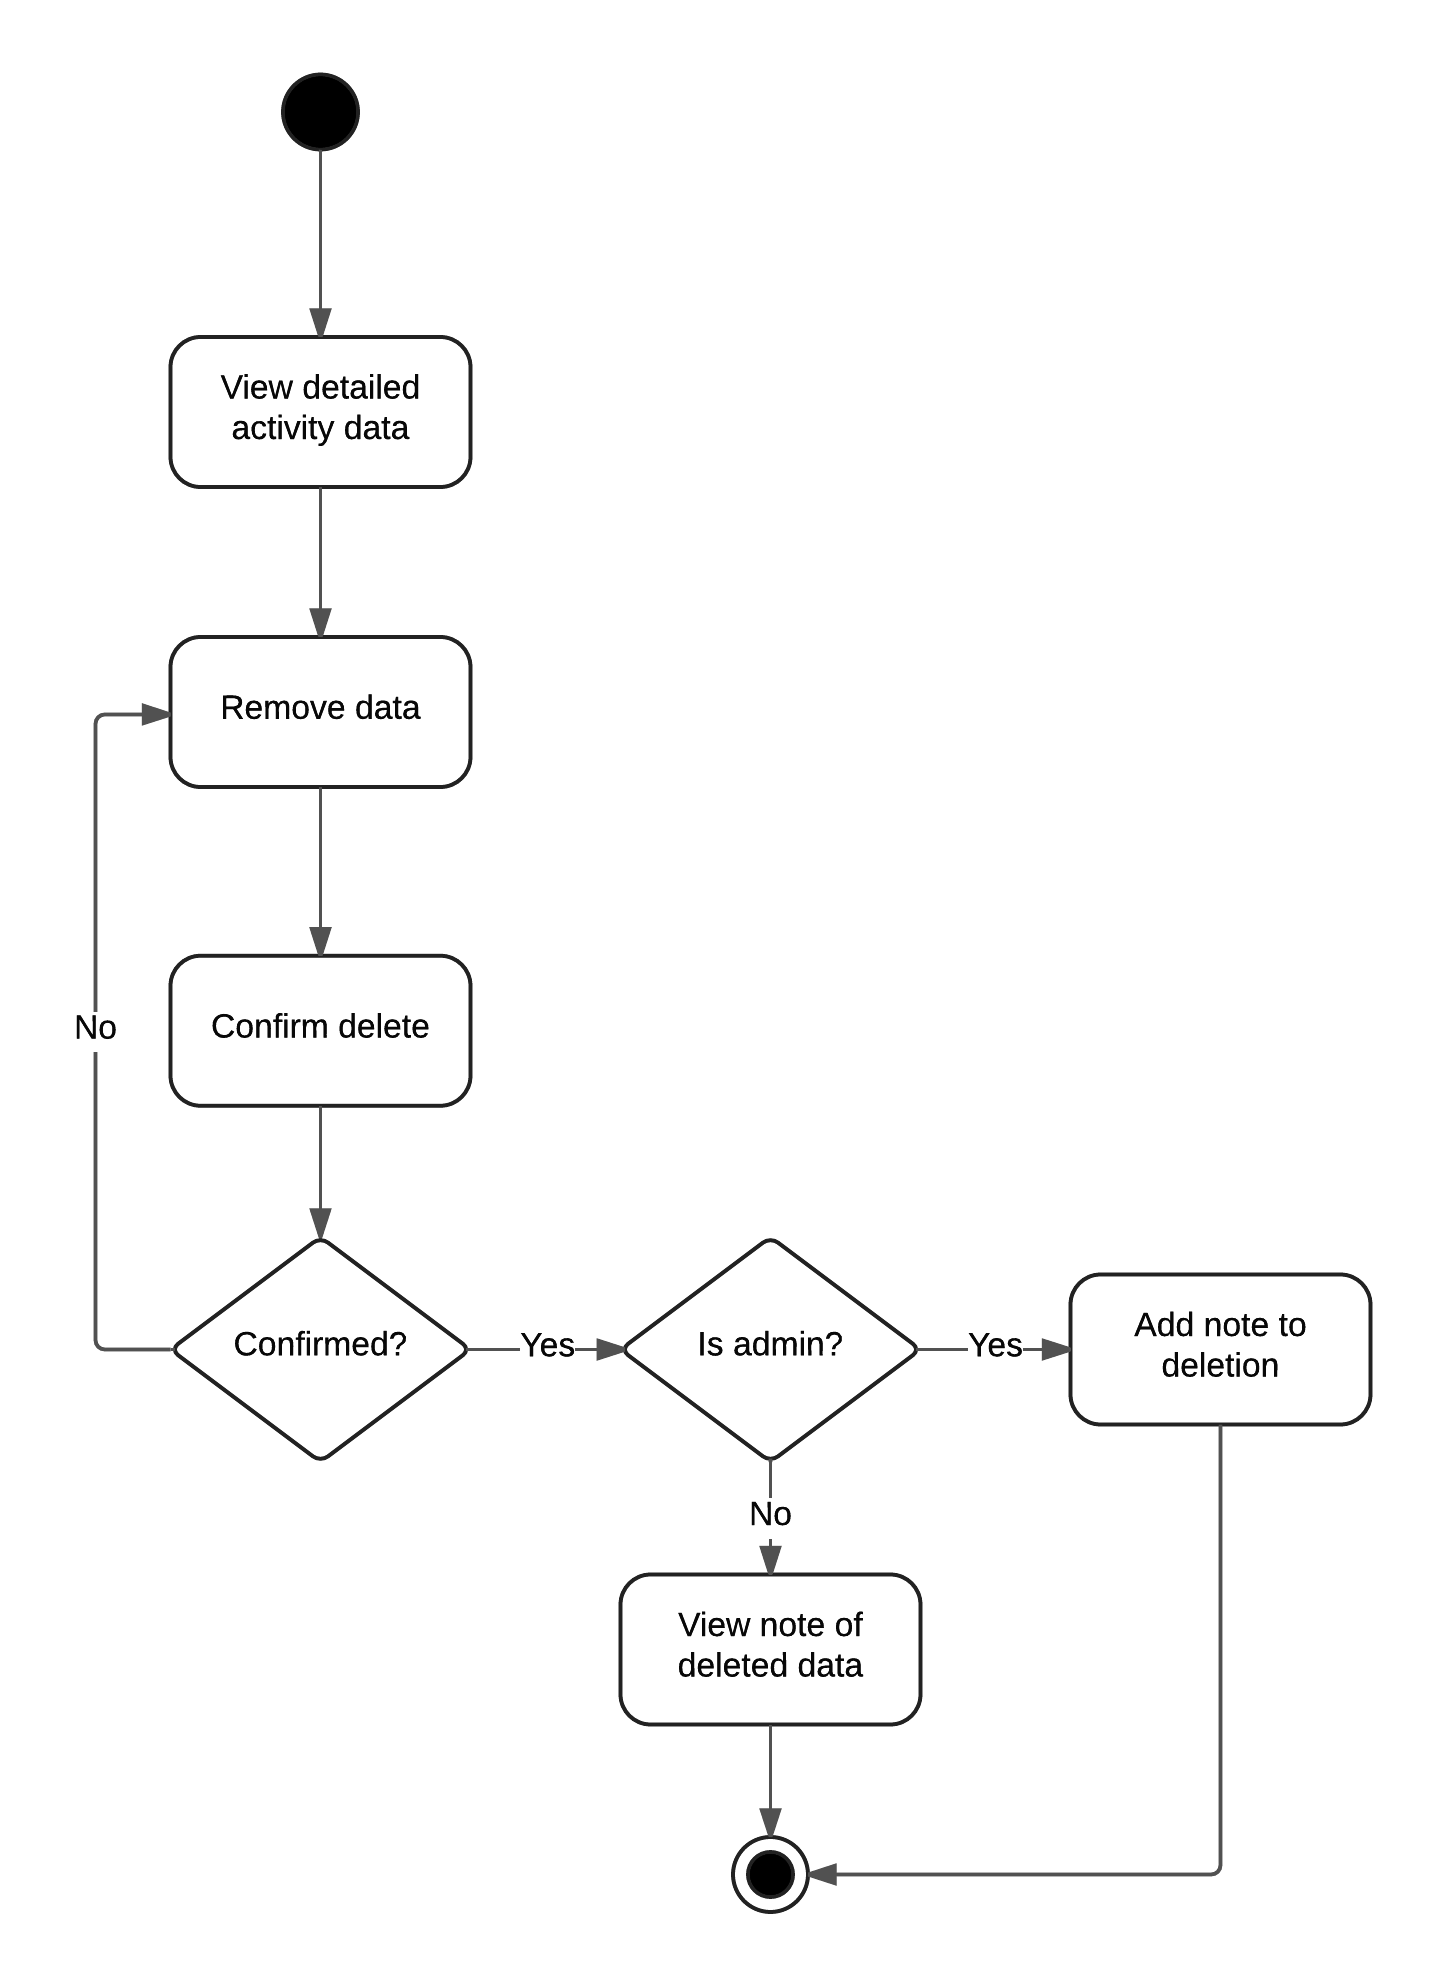
\includegraphics[width=0.4\textwidth]{../design/UML/StateActivity/Accessing-Removing-Activity-Data.png}
\caption{An activity diagram showing the states a participant/administrator passes through in order to delete activity data.}
\label{fig:activity-diagram-accessing-removing-activity-data}
\end{figure}

The next figure (\ref{fig:activity-diagram-device-authorisation}) shows the states of the workflow for authorising a users device (e.g. a Fitbit or Jawbone device) for use with our system. Users should be able to view which devices are connected to the system and revoke access when desired. They should also be able to add a new device and the system should handle if the external site returns a failure.

Group management activities are shown in figure \ref{fig:activity-diagram-group-management}. Most of these actions are fairly self explanatory but there is a slightly non-trivial case where we wish to add a user to the group. In this case we must check to make sure that they are removed from their old group as they can only ever be affiliated with one group at a time.

\begin{figure}[H]
\centering
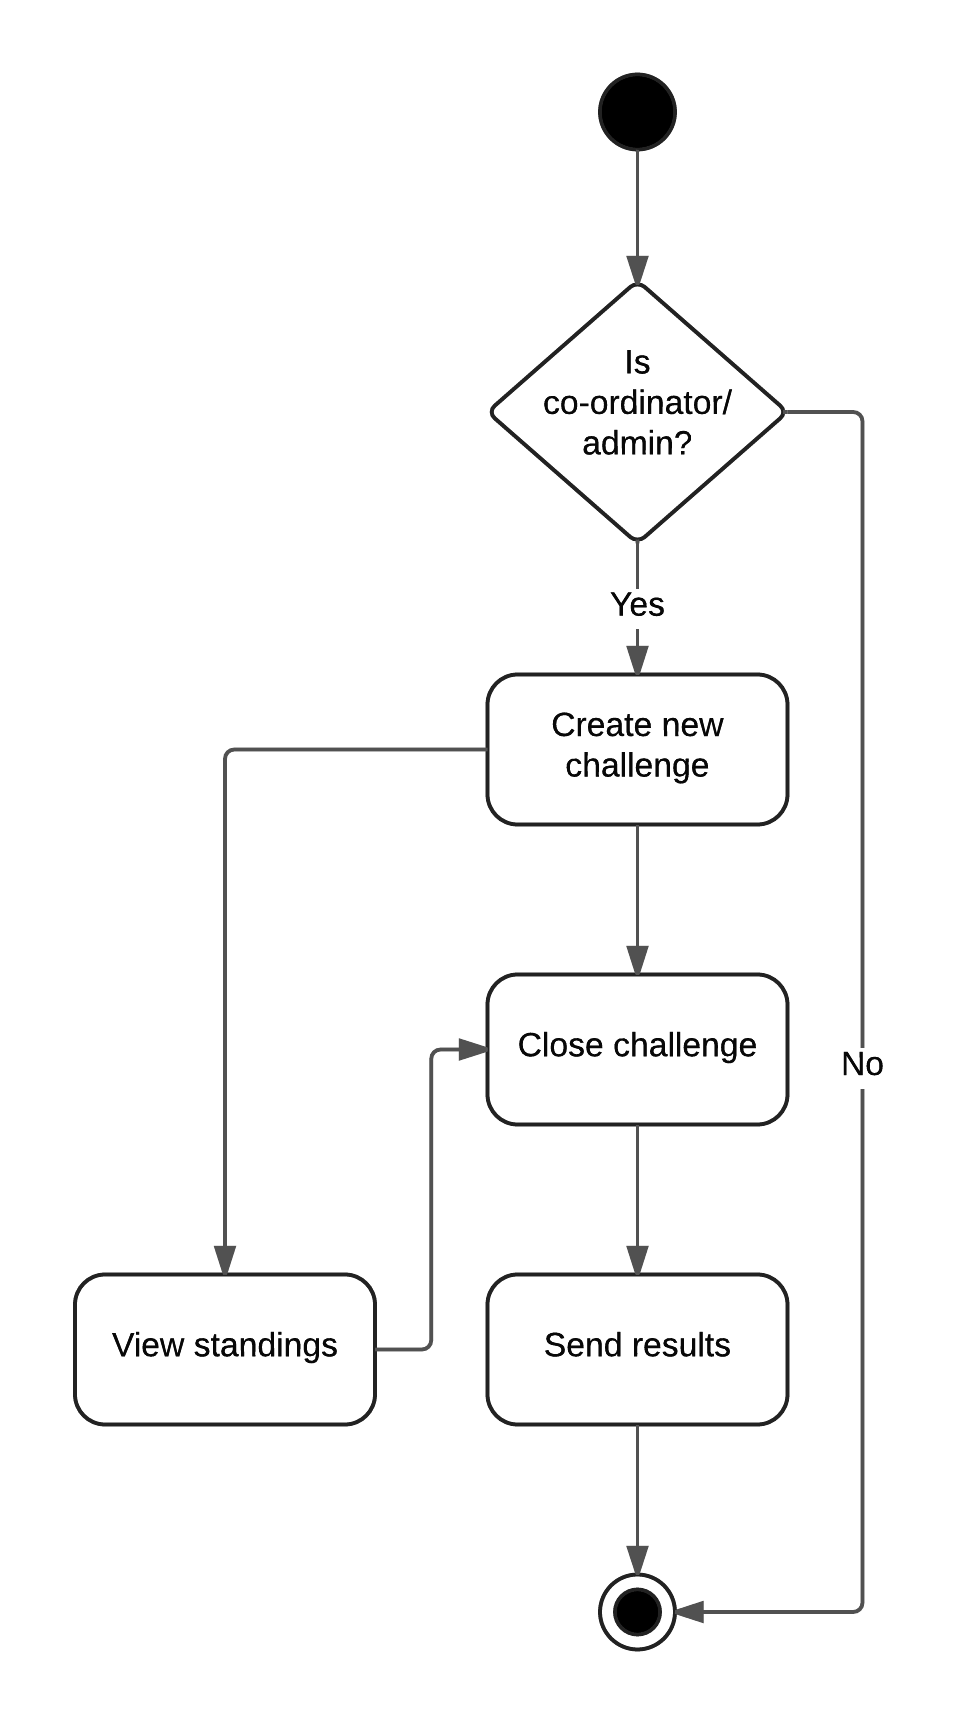
\includegraphics[width=0.4\textwidth]{../design/UML/StateActivity/Creating-Closing-Challenges.png}
\caption{An activity diagram showing the workflow for device authorisation.}
\label{fig:activity-diagram-device-authorisation}
\end{figure}

\begin{figure}[H]
\centering
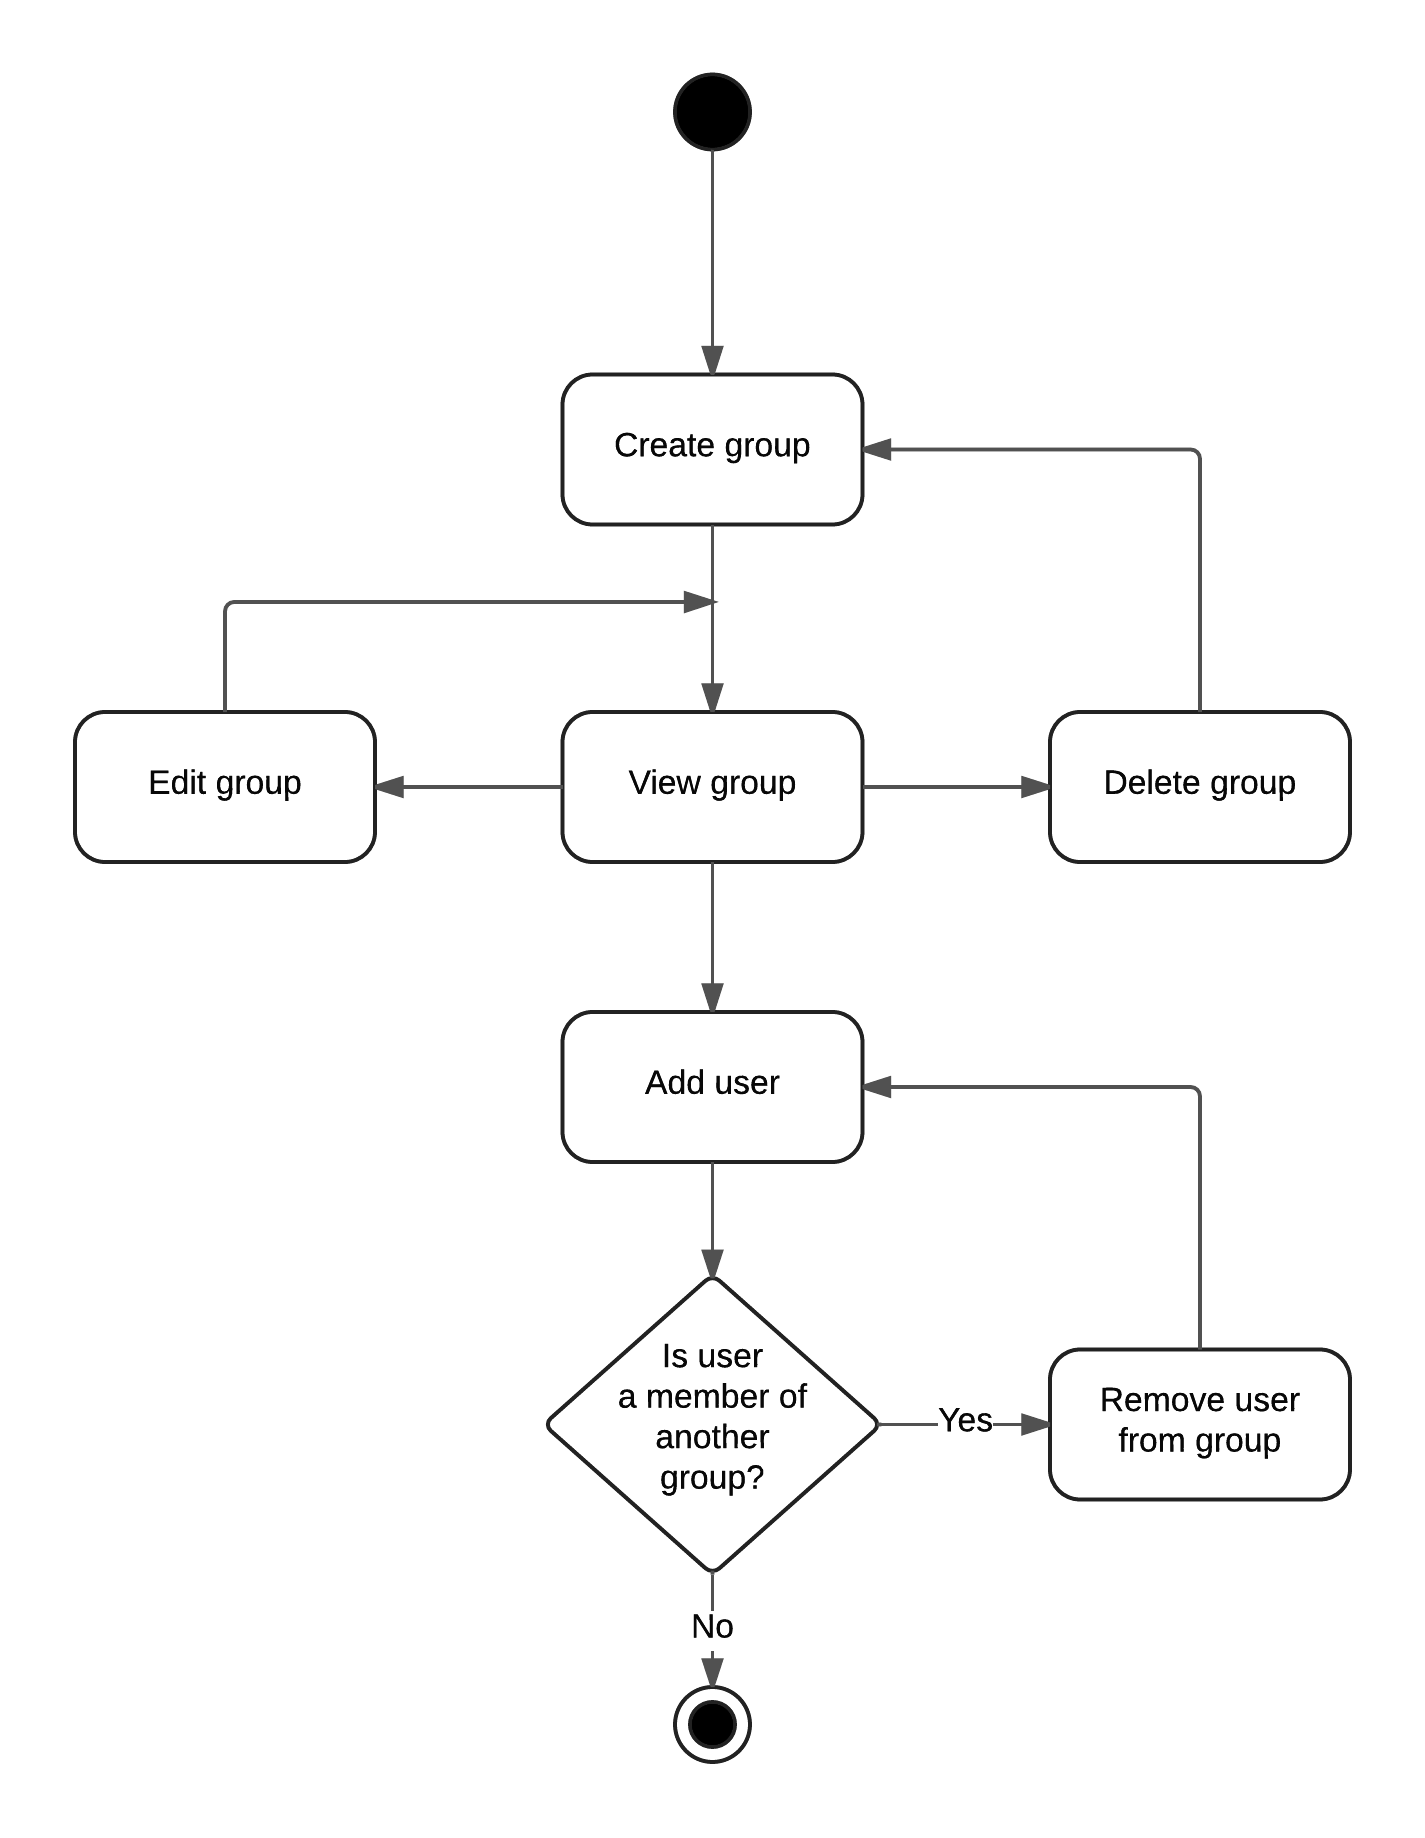
\includegraphics[width=0.4\textwidth]{../design/UML/StateActivity/Groups-Management.png}
\caption{An activity diagram for the management of user groups in GoAber.}
\label{fig:activity-diagram-group-management}
\end{figure}

In figure \ref{fig:activity-diagram-manual-api-data-input} the activity flow for entering data into the system is shown. Activity data can be entered manually by participants in which case their data is validated on submission. With external systems there is the potential possibility of a connection failure and that we get bad data back. This could be either from a device API or manual input for a third party device via the SOAP API. 

\begin{figure}[H]
\centering
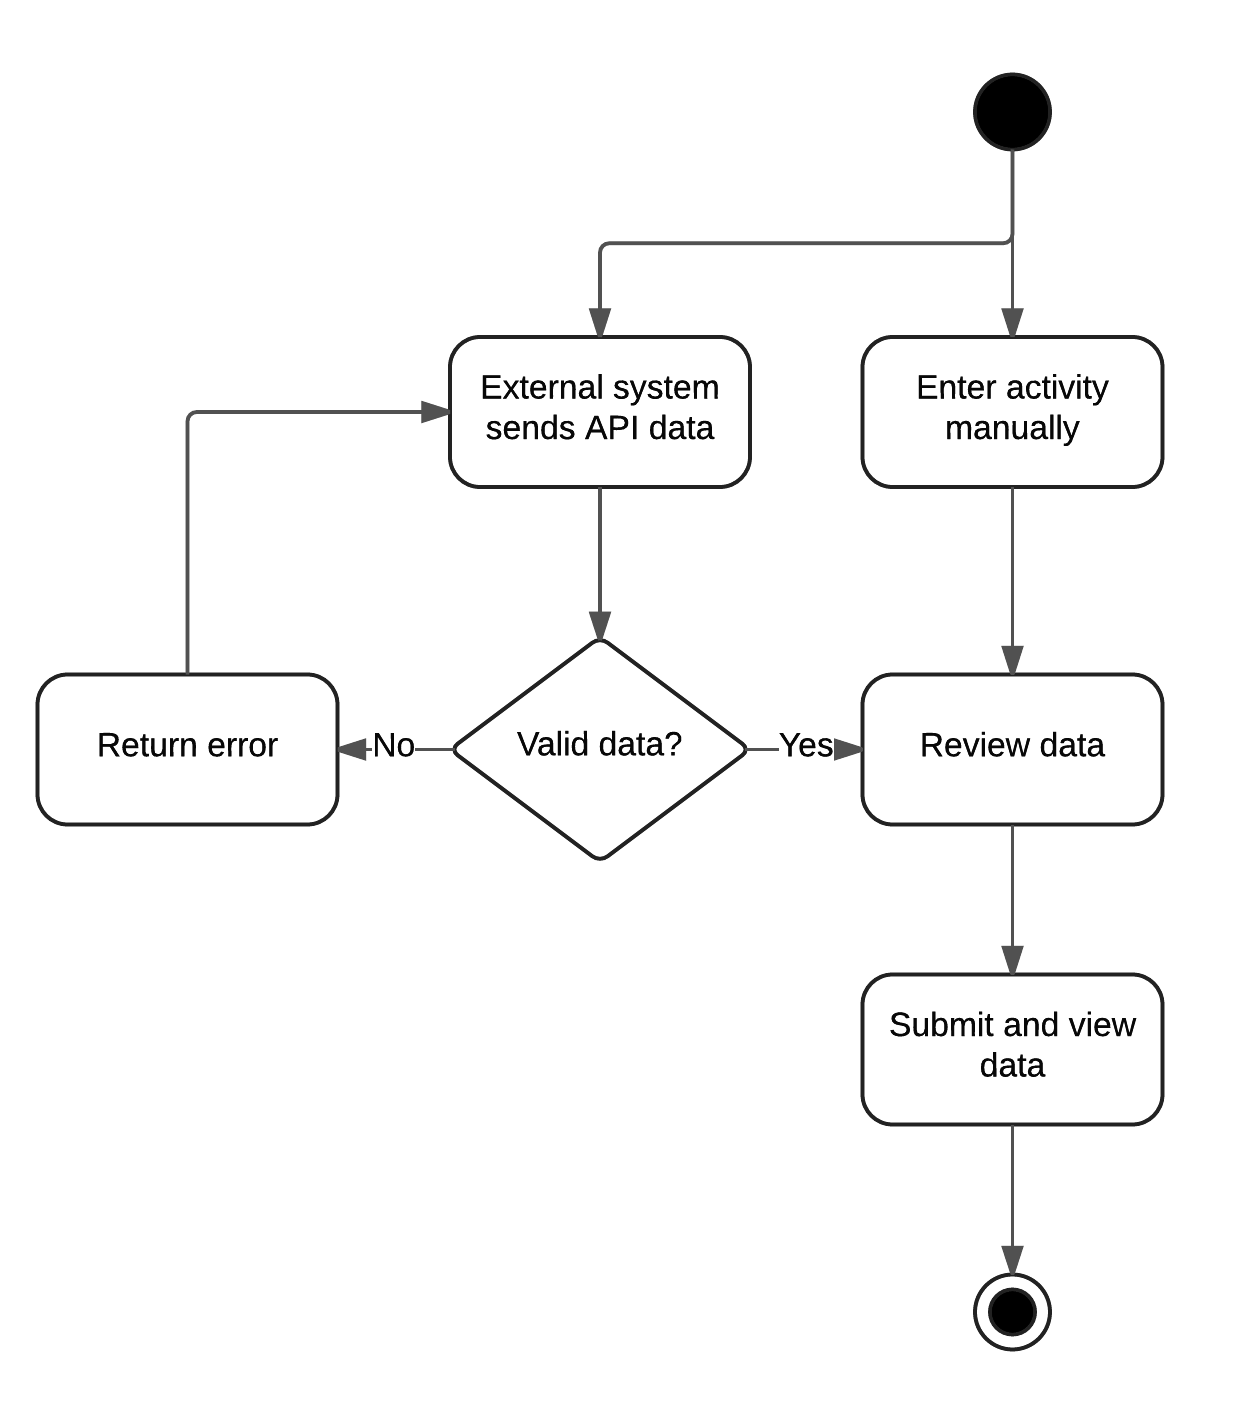
\includegraphics[width=0.4\textwidth]{../design/UML/StateActivity/Manual-API-Data-Input.png}
\caption{An activity diagram for manually inputting user data into the sytem.}
\label{fig:activity-diagram-manual-api-data-input}
\end{figure}



